% !TEX root = ../my-thesis.tex
%
\chapter{Data Analysis}
\label{sec:analysis}
This chapter will focus on the analysis of the research question. First, it will take a look at the standardised incidence rate in each country. Next, the relationship between the number of infections and several factors of interest will be analysed. For this analysis, a probability must be found that fits the data reasonably well. One way to do this is presented in Section~\ref{sec:likelihood}. Thereafter, two different types of models are calculated; models without a spatial component and models with a spatial component. Section~\ref{sec:nospatial} contains the results of the models without a spatial component and Section~\ref{ch:spatial} contains the results of the models with the spatial component. Next, it is analysed how the performance of the spatial models changes when changing the value for the standard deviation $\sigma_0$ in Equation~\ref{pcprec}.
\clearpage
\section{Standardised Incidence Ratio (SIR)}
This section takes a brief look at the SIR for the countries of interest. Recall from Equation~\ref{eq:sir}, that the SIR is defined as the ratio of observed counts to expected counts.
\subsection{SIR for Germany}
When looking at the SIR for Germany in Figure~\ref{sirgermany}, it is noticeable that the actual number of infections in the eastern parts of Germany, especially in Saxony, is considerably higher than the expected number of infections. Furthermore, parts of Bavaria have an increased SIR compared to the rest of Germany, excluding Saxony. This could be due to the fact that the regions share a border with the Czech Republic, a country that is substantially more affected by Covid-19 than Germany. The northern parts of Germany show the lowest SIR which is possibly due to the fact that this region is sparsely populated.
\begin{figure}[H]
 \centering
 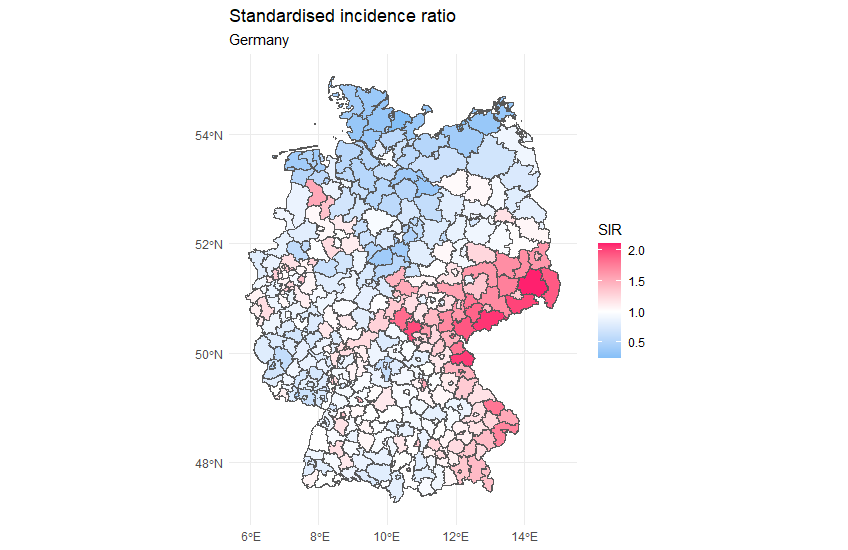
\includegraphics[width = 1.2\textwidth]{sir_germany.png}
 \caption{The SIR for Germany based on the data of the 2nd of May 2021}
 \label{sirgermany}
\end{figure}
\subsection{SIR for Norway}
Looking at the standardised incidence rate for Norway in Figure~\ref{sirnorway}, a standardised incidence rate of less than 1 can be seen for most municipalities north of Trondheim. In the southern parts of Norway there are several municipalities with a rate above 1, for example the standardised incidence rate around the capital Oslo is around 2. However, the two small municipalities, Hyllestad and Ulvik, have the highest standardised incidence rate in Norway. In Hyllestad, 95 of 1328 people have been infected with Covid-19 so far, while in Ulvik, 134 of 1080 people have been infected so far. \\
The SIR in Hyllestad is around 3.4, following an outbreak in a shipyard in autumn 2020 \autocite[][]{newspaper1}, while Ulvik has a ratio of around 5.7, following an outbreak of the UK variant of Covid-19. According to the head of the municipality, Hans Petter Thorbjørnsen, the infections are thought to have spread through children \autocite[][]{newspaper2}.
\begin{figure}[H]
 \centering
 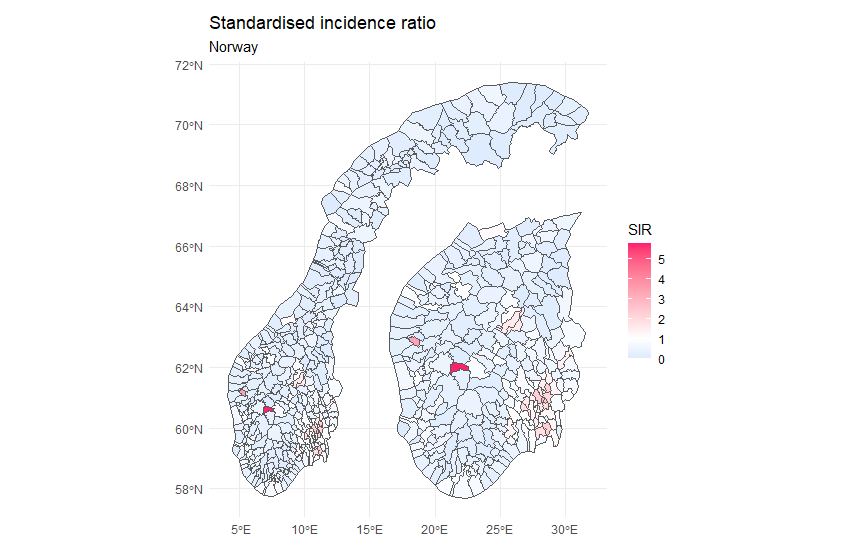
\includegraphics[width = 1.2\textwidth]{sir_norway.png}
 \caption{The SIR for Norway based on the data of the 2nd of May 2021}
 \label{sirnorway}
\end{figure}
Because the high numbers from two small municipalities complicate the interpretation of Figure~\ref{sirnorway}, Figure~\ref{sirnorwaylog} shows the SIR on a log10 scale. On this scale, a value of 0 means that the risk of infection in a given municipality is neither lower nor higher. Values below 0 mean that the risk of infection in a municipality is lower than average, while values above 1 mean that the risk of infection in a municipality is higher than average. It is now clearer that the standardized incidence ratio is below 1 in most parts of Norway, but that there is a higher risk in the region around Oslo.
\begin{figure}[H]
 \centering
 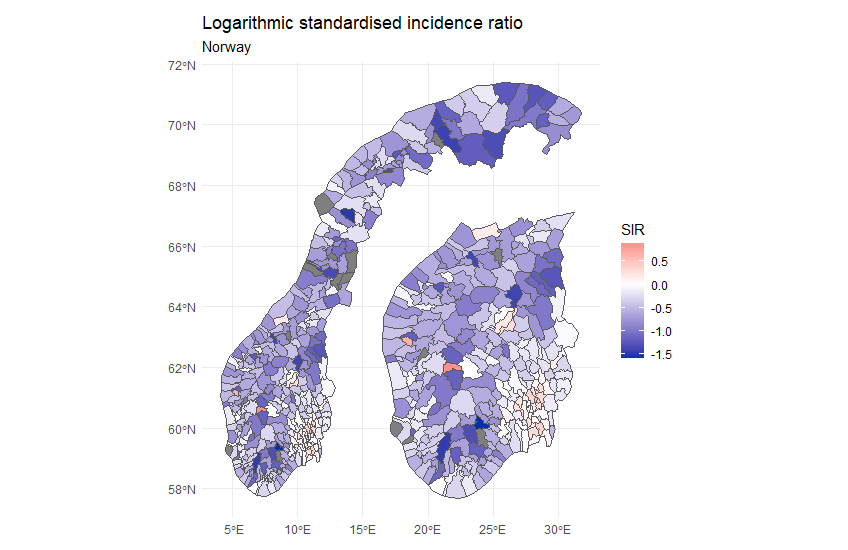
\includegraphics[width = 1.2\textwidth]{sir_norway_log.png}
 \caption{The log10 SIR for Norway based on the data of the 2nd of May 2021}
 \label{sirnorwaylog}
\end{figure}
\clearpage
\section{Data Modelling}
After looking at the standardised incidence rates for the countries of interest, the next step is to take a closer look at the current figures for the respective countries. Spatial models are used to try to extract the factors that cause some populations to be at higher risk than populations in other geographical regions. Three different types of models are used for each country:
\begin{itemize}
  \item[1.] Besags Proper Spatial Model
  \item[2.] A Leroux Model
  \item[3.] A BYM2 Model
\end{itemize}
All of these models are computed using the INLA \autocite[][]{rinla} R package. \\
To specify each type of model, the code shown in Listing~\ref{codeModels} can be used. \\
The measures introduced in Section~\ref{sec:performance}, namely the DIC, the WAIC, the CPO and the mean absolute error (MAE), are used to compare the models.\\
In addition to specifying what type of spatial model to use, if any, there is also the option of specifying a prior. \\
As can be seen in Section~\ref{sec:pc_prior}, a pc prior can be specified for the precision parameter $\tau$, which is what is done here. \\
For the parameters $\sigma_0$ and $\alpha$ in Equation~\ref{eq:pc_prior_prec} the values 1 and 0.01 are chosen. \\
The models are compared using the mean absolute error. For this, 20\% of the observations are removed from the training set and used for testing instead. The predicted number of infections for these municipalities is then compared to the actual numbers.
\subsection{Choice of Likelihood}\label{sec:likelihood}
Before the models are computed, however, the distribution that fits the number of cases must first be found. One way to do this, the function \texttt{descdist()} from the \texttt{fitdistrplus} R package is used. The Cullen and Frey graph illustrates how "close" a sample is to a theoretical distribution based on the kurtosis and the square of the skewness, defined in Equation~\ref{eq:kurtosis} and Equation~\ref{eq:skewness}. It can be used to get a preliminary idea of which distributions fit the data, in this case the number of infections, reasonably well. \\
The plots for Germany and Norway can be seen in Figure~\ref{cf_germany} and Figure~\ref{cf_norway}. The blue dot represents the data, the star a theoretical normal distribution, the dashed line a theoretical Poisson distribution and the grey area a theoretical negative binomial distribution. In both cases, the blue dot is relatively far from the star and lies in the region of a negative binomial distribution. For the Norwegian sample shown in Figure~\ref{cf_norway}, the sample is closer to a Poisson distribution than is the case for the German sample in Figure~\ref{cf_germany}.
\begin{figure}[H]
  \centering
  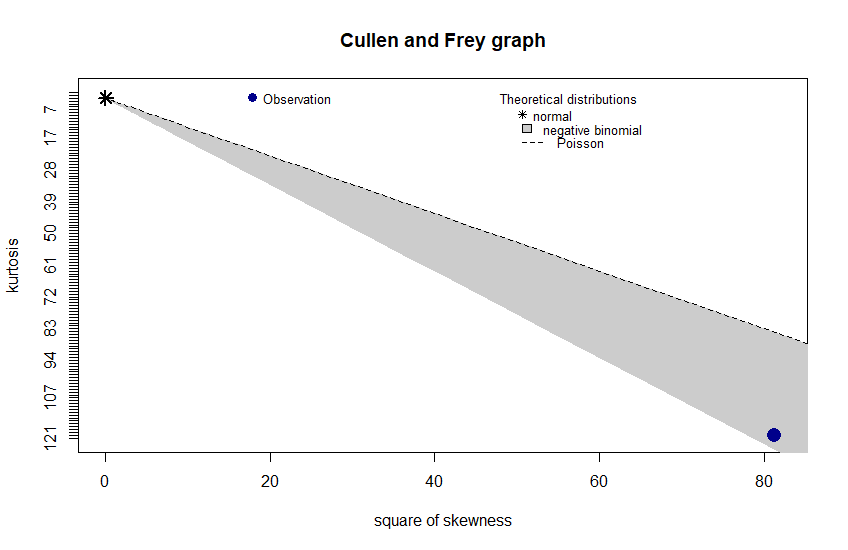
\includegraphics[width = 0.8\textwidth]{cf_germany.png}
  \caption{The Cullen and Frey graph for Germany}
  \label{cf_germany}
\end{figure}
\begin{figure}[H]
  \centering
  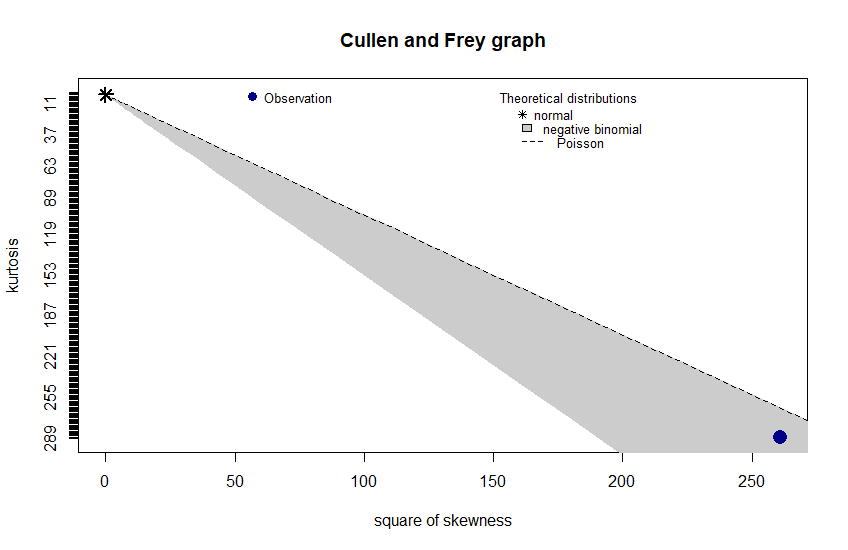
\includegraphics[width = 0.8\textwidth]{cf_norway.png}
  \caption{The Cullen and Frey graph for Norway}
  \label{cf_norway}
\end{figure}
Next, a negative binomial distribution, a normal distribution, and a Poisson distribution are fitted to the data using the maximum likelihood method. The negative binomial fits for both countries can be seen in Figure~\ref{fitNegbinomGermany} and Figure~\ref{fitNegbinomNorway}. The fits for the normal and Poisson distribution for both countries, are shown in the Appendix in Figure~\ref{fitNormalGermany}, Figure~\ref{fitPoissonGermany}, Figure~\ref{fitNormalNorway} and Figure~\ref{fitPoissonNorway}. \\
The QQ-plot for Germany and Norway looks quite similar, as there appears to be a linear relationship between the theoretical quantile and the sample quantiles, up to a certain point where the sample quantiles have a higher value than the theoretical quantiles, indicating that the distribution is right skewed. Since there are many municipalities with relatively few cases and few municipalities with a large number of cases, this is to be expected. It can also be seen that the empirical cumulative density function closely follows the theoretical cumulative density function.
\begin{figure}[H]
  \centering
  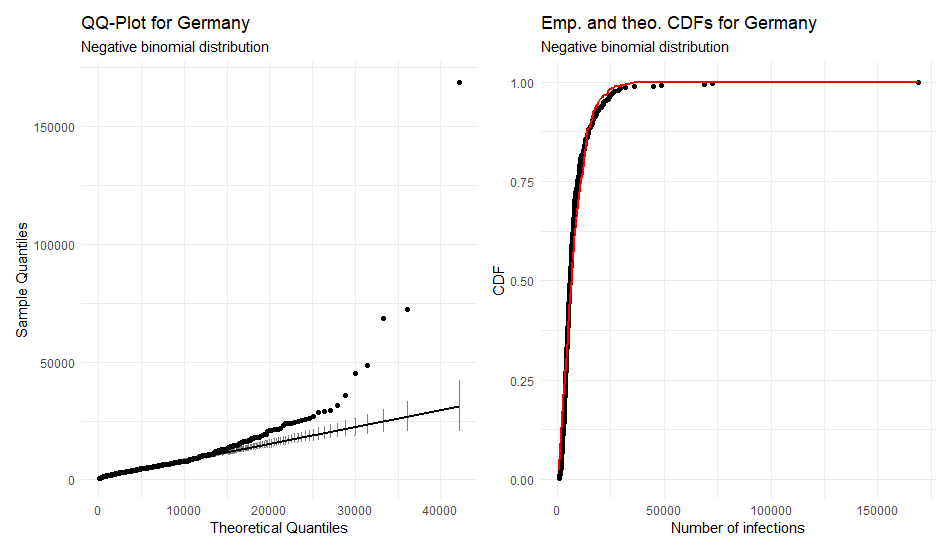
\includegraphics[width = 0.8\textwidth]{fit_nbinom_germany.png}
  \caption{A negative binomial fit to the number of cases in German municipalities}
  \label{fitNegbinomGermany}
\end{figure}
\begin{figure}[H]
  \centering
  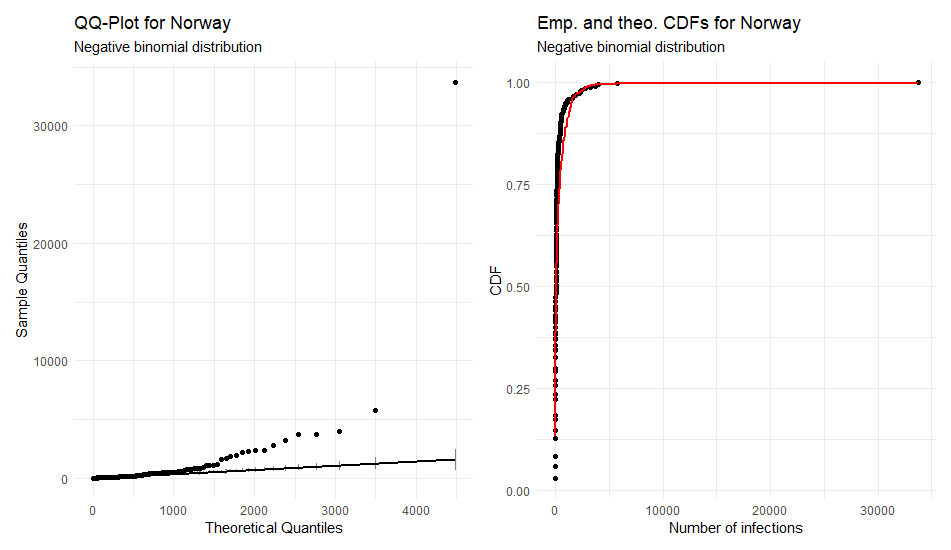
\includegraphics[width = 0.8\textwidth]{fit_nbinom_norway.png}
  \caption{A negative binomial fit to the number of cases in Norwegian municipalities}
  \label{fitNegbinomNorway}
\end{figure}
Lastly, the AIC is calculated for fitting a normal distribution to the data, a Poisson distribution to the data and a negative binomial distribution to the data. The values can be seen in Table~\ref{aic}. Afterwards, the negative binomial distribution is chosen as the distribution of the target variable in both cases. \\
\begin{table}[H] 
\caption{The AIC for different distributions for Germany and Norway \label{aic}}
\begin{tabular}{l l r}
\toprule
\textbf{Country}	& \textbf{Distribution}	& \textbf{AIC} \\
\midrule
Germany & Normal & 8619 \\
Germany & Poisson & 2699357 \\
Germany & Negative Binomial & 8010 \\
Norway & Normal & 6400 \\
Norway & Poisson & 509139 \\
Norway & Negative Binomial & 4293 \\
\bottomrule
\end{tabular}
\end{table} 
The poor fit for the Poisson distribution can be explained by looking at the range of the number of confirmed cases in a given municipality. For Germany, this number ranges from 697 to 169021 (as of May 2, 2021), while for Norway, the number ranges from 0 to 34654 (as of May 2, 2021). This results in a mean and standard deviation for Germany of 8550 and 11204, respectively. For Norway, the values for these metrics are 326 and 1930. This is problematic because, as shown in Equation~\ref{eq:poisson_exp} and Equation~\ref{eq:poisson_var}, for a Poisson distribution the expected value and the variance should be equal. \\
Looking at a histogram for the confirmed number of cases and overlaying the densities of a normal, Poisson and a negative binomial distribution helps to confirm the choice of a negative binomial distribution as the distribution that the data most closely resembles. Figure~\ref{fitDistrGermany} and Figure~\ref{fitDistrNorway} both show that a negative binomial distribution fits the data better than a normal distribution. Due to the high values for the AIC, the Poisson distribution is excluded from these graphics.
\begin{figure}[H]
  \centering
  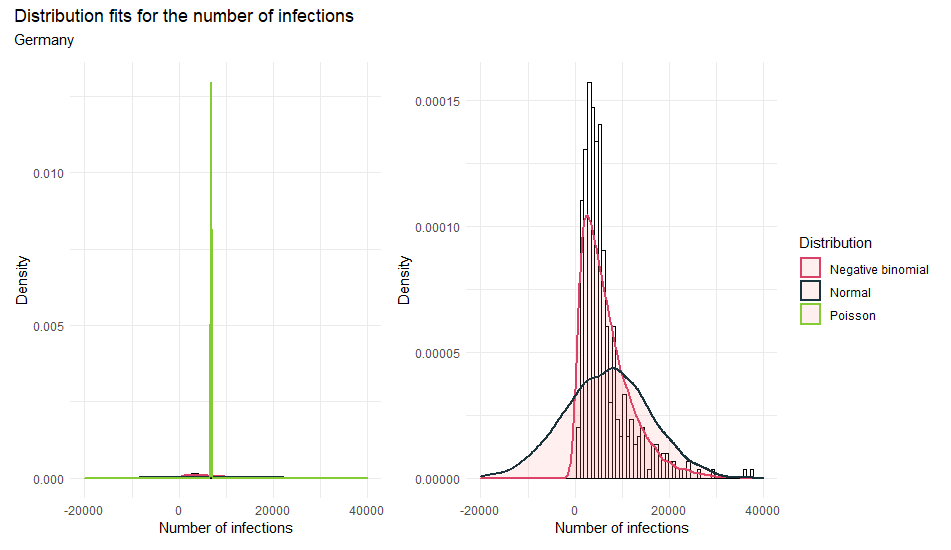
\includegraphics[width = 0.8\textwidth]{distrfit_germany.png}  
  \caption{Histogram for the number of cases in German municipalities with a normal and a negative binomial distribution overlayed.}
  \label{fitDistrGermany}
\end{figure}
\begin{figure}[H]
  \centering
  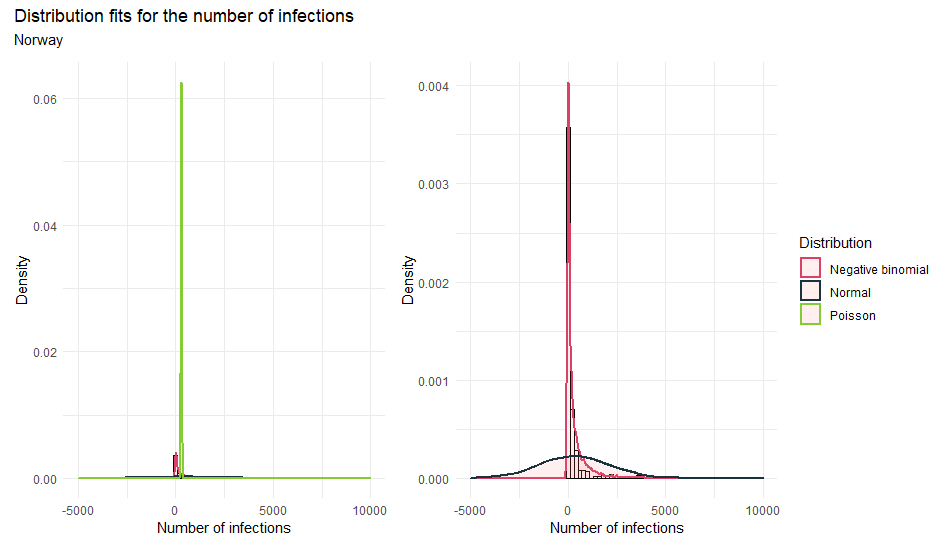
\includegraphics[width = 0.8\textwidth]{distrfit_norway.png}
  \caption{Histogram for the number of cases in Norwegian municipalities with a normal and a negative binomial distribution overlayed.}
  \label{fitDistrNorway}
\end{figure}
\clearpage
\section{Models without a Spatial Component}\label{sec:nospatial}
To establish a baseline, a look is first taken at models that do not include a spatial effect. This way, it can be observed how the means and credibility intervals of the covariates change when a spatial effect is added to a model and how the performance of the model changes with respect to the goodness-of-fit indicators introduced in Section~\ref{sec:performance}. \\
Before computing the models, using the $\hbox{VIF}$ introduced in Section~\ref{sec:vif}, predictors are removed if their $\hbox{VIF}$ is above 5. To do this, a GLM is first run on all variables, followed by the calculation of $\hbox{VIF}$. Then the variable with the highest value is removed before running the model again with all remaining variables. This process is repeated until only variables with a $\hbox{VIF}$ of less than 5 remain. \\
In sections~\ref{sec:nospatial_germany} and~\ref{sec:nospatial_norway} the results of these models are presented. Their goodness-of-fit indicators as well as the coefficients together with their credibility intervals calculated as in section~\ref{sec:mean_iv} are reported. \\
These models are based on data from 2 May 2021, when 3,428,487 people were infected with Covid-19 in Germany, while 87,537 people were infected in Norway. The five municipalities with the most infections in Germany are shown in Table~\ref{top5germany} and in Table~\ref{top5norway} for Norway.
\begin{table}[H] 
\caption{The German municipalities with the most infections as of May 2nd 2021. \label{top5germany}}
\begin{tabular}{l r r}
\toprule
\textbf{Municipality}	& \textbf{Population}	& \textbf{Number of infections} \\
\midrule
SK Berlin & 3644826 & 169021  \\   
SK Hamburg & 1841179 & 72595  \\
SK Munich & 1471508 & 68762  \\
SK Cologne & 1085664 & 48831  \\
Region Hannover & 1157624 & 45043  \\
\bottomrule
\end{tabular}
\end{table}
\begin{table}[H] 
\caption{The Norwegian municipalities with the most infections as of May 2nd 2021. \label{top5norway}}
\begin{tabular}{l r r r}
\toprule
\textbf{Municipality}	& \textbf{Population}	& \textbf{Number of infections} &\textbf{\% first vaccine shot} \\
\midrule
Oslo & 693494 & 34654 & 32.7\%\\
Bergen & 283929 & 6039 & 30.0\%\\
Drammen & 101386 & 4097 & 34.1\%\\
Bærum & 127731 & 3860 & 31.7\%\\
Lillestrøm & 85983 & 3819 & 30.2\%\\
\bottomrule
\end{tabular}
\end{table}
\subsection{Models without a Spatial Component for Germany}\label{sec:nospatial_germany}
Table~\ref{allGermany_nospatial} contains the performance measures for the baseline model for Germany, while Table~\ref{FixedAllGermany_nospatial} contains the posterior mean, the exponentiated posterior mean and the credibility intervals of the coefficients. It can be seen that the intercept as well as six of the coefficients are significant.
\begin{table}[H] 
\caption{The performance measures for the model without a spatial component. \label{allGermany_nospatial}}
\begin{tabular}{r r r r r}
\toprule
\textbf{DIC}	& \textbf{WAIC} & \textbf{CPO} & \textbf{$\hbox{MAE}_{\hbox{train}}$} & \textbf{$\hbox{MAE}_{\hbox{test}}$}\\
\midrule
5593 & 5596 & -2814 & 1434 & 1284 \\
\bottomrule
\end{tabular}
\end{table}
\begin{table}[H]
\caption{The fixed effects for the model. Values are rounded. A $^*$ denotes a significant effect. \label{FixedAllGermany_nospatial}}
\begin{tabular}{l r r r r c}
\toprule
\textbf{Variable}	& \textbf{mean$_{\hbox{p}}$}	& \textbf{exp(mean$_{\hbox{p}}$)} & \textbf{exp(q0025$_{\hbox{p}}$)} & \textbf{exp(q0975$_{\hbox{p}}$)} & \textbf{sig.}\\
\midrule
(Intercept) & -0.041 & 0.960 & 0.937 & 0.985 & $^*$\\
AfD & 0.172 & 1.190 & 1.057 & 1.335 & $^*$\\
Population & \multirow{2}{*}{0.164} & \multirow{2}{*}{1.178} & \multirow{2}{*}{1.127} & \multirow{2}{*}{1.232} & \multirow{2}{*}{$^*$}\\
density \\
Logarithmic & \multirow{2}{*}{0.082} & \multirow{2}{*}{1.086} & \multirow{2}{*}{1.039} & \multirow{2}{*}{1.134} & \multirow{2}{*}{$^*$}\\
trade tax \\
Platform & 0.037 & 1.038 & 0.988 & 1.089 \\
Die Union & 0.026 & 1.029 & 0.893 & 1.180\\
Higher & \multirow{2}{*}{0.018} & \multirow{2}{*}{1.018} & \multirow{2}{*}{0.981} & \multirow{2}{*}{1.058} \\
Education\\
Sex & 0.017 & 1.018 & 0.986 & 1.050 & \\
Urban density & 0.009 & 1.009 & 0.973 & 1.047 \\
FDP & 0.005 & 1.005 & 0.971 & 1.041 \\
Place of & \multirow{2}{*}{-0.010} & \multirow{2}{*}{0.991} & \multirow{2}{*}{0.951} & \multirow{2}{*}{1.031} \\
worship\\
Clinic & -0.011 & 0.990 & 0.942 & 1.041 \\
Nursing & \multirow{2}{*}{-0.013} & \multirow{2}{*}{0.987} & \multirow{2}{*}{0.958} & \multirow{2}{*}{1.018} \\
home\\
Office & -0.031 & 0.970 & 0.929 & 1.013 \\
Marketplace & -0.044 & 0.957 & 0.905 & 1.012 \\
SPD & -0.091 & 0.914 & 0.847 & 0.984 & $^*$\\
The left & -0.119 & 0.888 & 0.822 & 0.958 & $^*$\\
Greens & -0.156 & 0.857 & 0.753 & 0.970 & $^*$\\
\bottomrule
\end{tabular}
\end{table}
\subsection{Models without a Spatial Component for Norway}\label{sec:nospatial_norway}
Table~\ref{allNorway_nospatial} contains the performance measures for the baseline model for Germany, while Table~\ref{fixedAllNorway_nospatial} contains the posterior mean, the exponentiated posterior mean and the credibility intervals of the coefficients. It can be seen that the intercept as well as four of the coefficients are significant.
\begin{table}[H] 
\caption{The performance measures for the model without a spatial component. \label{allNorway_nospatial}}
\begin{tabular}{r r r r r}
\toprule\textbf{DIC}	& \textbf{WAIC} & \textbf{CPO} & \textbf{$\hbox{MAE}_{\hbox{train}}$} & \textbf{$\hbox{MAE}_{\hbox{test}}$}\\
\midrule
2859 & 2864 & -703 & 229 & 92 \\
\bottomrule
\end{tabular}
\end{table} 
\begin{table}[H]
\caption{The fixed effects for the model. Values are rounded. A $^*$ denotes a significant effect. \label{fixedAllNorway_nospatial}}
\begin{tabular}{l r r r r c}
\toprule
\textbf{Variable}	& \textbf{mean$_{\hbox{p}}$}	& \textbf{exp(mean$_{\hbox{p}}$)} & \textbf{exp(q0025$_{\hbox{p}}$)} & \textbf{exp(q0975$_{\hbox{p}}$)} & \textbf{sig.}\\
\midrule
(Intercept) & -0.809 & 0.446 & 0.409 & 0.486 & $^*$ \\
Total & \multirow{2}{*}{0.237}& \multirow{2}{*}{1.270}& \multirow{2}{*}{1.112}& \multirow{2}{*}{1.446}& \multirow{2}{*}{$^*$}\\
immigrants \\
Unemployed & \multirow{2}{*}{0.233} & \multirow{2}{*}{1.266} & \multirow{2}{*}{1.084} & \multirow{2}{*}{1.474} & \multirow{2}{*}{$^*$} \\
immigrants\\
Urban density & 0.181 & 1.202 & 1.037 & 1.408 & $^*$ \\
Vaccinations & 0.055 & 1.058 & 0.947 & 1.179\\
Marketplace & 0.043 & 1.045 & 0.954 & 1.155 \\
Total & \multirow{2}{*}{0.037} & \multirow{2}{*}{1.043} & \multirow{2}{*}{0.852} & \multirow{2}{*}{1.269} \\
unemployment \\
Platform & 0.035 & 1.038 & 0.903 & 1.196 \\
Nursing & \multirow{2}{*}{0.006} & \multirow{2}{*}{1.007} & \multirow{2}{*}{0.930} & \multirow{2}{*}{1.106} \\
home\\
Higher & \multirow{2}{*}{0.004}& \multirow{2}{*}{1.005}& \multirow{2}{*}{0.928}& \multirow{2}{*}{1.105}\\ 
education \\
Median age & -0.028 & 0.974 & 0.864 & 1.093 \\
Place of\_ & \multirow{2}{*}{-0.035}& \multirow{2}{*}{0.968}& \multirow{2}{*}{0.840}& \multirow{2}{*}{1.118} \\
worship \\
Office & -0.146 & 0.867 & 0.741 & 1.013 \\
Sex & -0.175 & 0.840 & 0.748 & 0.941 & $^*$ \\
\bottomrule
\end{tabular}
\end{table}
\clearpage
\section{Spatial Models}\label{ch:spatial}
Looking at the SIR value for Germany in Figure~\ref{sirgermany} and the SIR value for Norway in Figure~\ref{sirnorway} and Figure~\ref{sirnorwaylog}, it clearly looks like there is a correlation between the SIR and the spatial units. For Germany, the SIR is higher in eastern Germany than in the rest of the country and in Norway the risk seems to be mainly concentrated around the Oslo region. \\
To check whether there is spatial autocorrelation, Moran's I, introduced in Section~\ref{sec:moran}, can be calculated and the Moran test can then be used to tell whether there is spatial autocorrelation. Under the null hypothesis of no spatial autocorrelation, a p-value greater than 0.05 would be expected. The results of the test are presented in Table~\ref{moranTest}. Looking at the p-value for both countries, it can be seen that the number of infections in a municipality and the spatial units are correlated.
\begin{table}[H] 
\caption{Results of the Moran test for Germany and Norway. \label{moranTest}}
\begin{tabular}{l r r r r}
\toprule
\textbf{Country} & \textbf{Moran's I}	& \textbf{$\mathbb{E}\left[I\right]$}	& \textbf{p-Value} \\
\midrule
Germany & 0.110 & -0.003 & < 0.01 \\
Norway & 0.110 & -0.003 & < 0.01 \\
\bottomrule
\end{tabular}
\end{table}
Therefore, after the models without spatial effect have been calculated and established as baseline models, a spatial term is added to the models calculated in Section~\ref{sec:nospatial} , in order to model this spatial correlation.
\subsection{Spatial Models for Germany}\label{sec:spatial_germany}
Looking at the performance of the spatial models and the model with the spatial component shown in Table~\ref{allGermany}, it can be seen that the spatial models perform better in terms of the DIC, WAIC and MAE, while they perform equally well or better in terms of the CPO. \\
The best performance of all models, in terms of MAE, was observed for the Besag model, just ahead of the BYM2 model.
\begin{table}[H] 
\caption{The performance measures for the best performing model of each type. \label{allGermany}}
\begin{tabular}{l r r r r r}
\toprule
\textbf{Model}	& \textbf{DIC}	& \textbf{WAIC} & \textbf{CPO} & \textbf{$\hbox{MAE}_{\hbox{train}}$} & \textbf{$\hbox{MAE}_{\hbox{test}}$}\\
\midrule
No spatial & 5593 & 5596 & -2814 & 1434 & 1284 \\
Besag& 4842 & 4897 & -2784 & 143 & 1027\\
BYM2 & 4747 & 4806 & -2781 & 103 & 1043\\
Leroux & 4830 & 4843 & -2966 & 88 & 1264 \\
\bottomrule
\end{tabular}
\end{table}
Figure~\ref{intervalGermany} shows the differences between the coefficients in the model without the spatial component and the BYM2 model. Excluding the intercept, only three effects are significant in the BYM2 model compared to six in the model without the spatial component. Moreover, the coefficients of the BYM2 model are closer to 1. 
\begin{figure}[H]
  \centering
  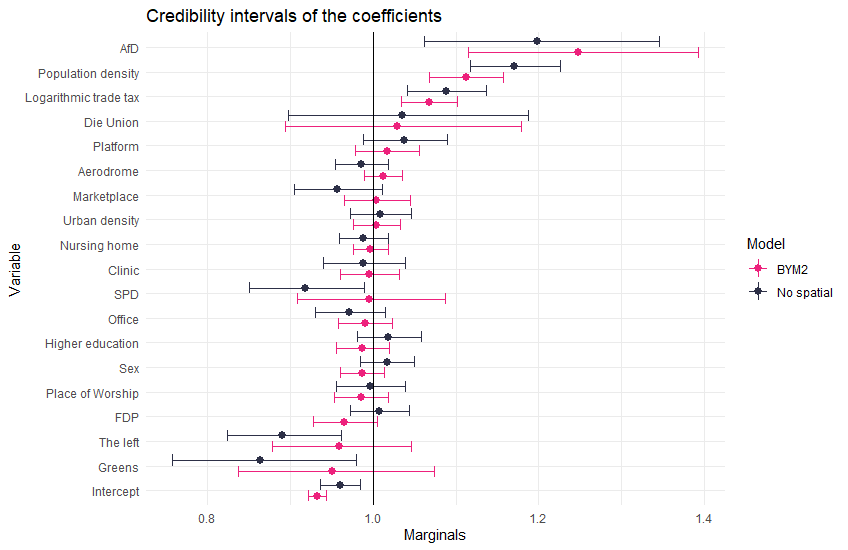
\includegraphics[width = \textwidth]{intervals_germany.png}
  \caption{The posterior mean and credibility intervals of the coefficients}
  \label{intervalGermany}
\end{figure}
The values of the coefficients and credibility intervals are shown in Table~\ref{FixedAllGermany_spatial}.
\begin{table}[H]
\caption{The fixed effects for the model. Values are rounded. A $^*$ denotes a significant effect. \label{FixedAllGermany_spatial}}
\begin{tabular}{l r r r r c}
\toprule
\textbf{Variable}	& \textbf{mean$_{\hbox{p}}$}	& \textbf{exp(mean$_{\hbox{p}}$)} & \textbf{exp(q0025$_{\hbox{p}}$)} & \textbf{exp(q0975$_{\hbox{p}}$)} & \textbf{sig.}\\
\midrule
(Intercept) & -0.070 & 0.932 & 0.922 & 0.944 & $^*$\\
AfD & 0.227 & 1.257 & 1.122 & 1.402 & $^*$\\
Population & \multirow{2}{*}{0.103} & \multirow{2}{*}{1.109} & \multirow{2}{*}{1.065} & \multirow{2}{*}{1.154} & \multirow{2}{*}{$^*$}\\
density \\
Logarithmic & \multirow{2}{*}{0.066} & \multirow{2}{*}{1.068} & \multirow{2}{*}{1.035} & \multirow{2}{*}{1.102} & \multirow{2}{*}{$^*$}\\
trade tax \\
Die Union & 0.037 & 1.041 & 0.904 & 1.192\\
Platform & 0.015 & 1.015 & 0.977 & 1.054 \\
Marketplace & 0.004 & 1.004 & 0.964 & 1.045 \\
Urban density & 0.003 & 1.003 & 0.974 & 1.032 \\
SPD & 0.001 & 1.002 & 0.915 & 1.095\\
Nursing& \multirow{2}{*}{-0.002} & \multirow{2}{*}{0.998} & \multirow{2}{*}{0.977} & \multirow{2}{*}{1.020} \\
Home\\
Clinic & -0.006 & 0.994 & 0.959 & 1.031 \\
Office & -0.008 & 0.992 & 0.960 & 1.025 \\
Place of & \multirow{2}{*}{-0.011} & \multirow{2}{*}{0.989} & \multirow{2}{*}{0.959} & \multirow{2}{*}{1.021} \\
Worship\\
Sex & -0.014 & 0.987 & 0.960 & 1.014 & \\
Higher & \multirow{2}{*}{-0.015} & \multirow{2}{*}{0.985} & \multirow{2}{*}{0.954} & \multirow{2}{*}{1.017} \\
Education\\
FDP & -0.030 & 0.971 & 0.933& 1.009 \\
The left & -0.036 & 0.966 & 0.884 & 1.053\\
Greens & -0.045 & 0.958 & 0.844 & 1.082 \\
\bottomrule
\end{tabular}
\end{table}
For the hyperparameters, a value of 19.75 is reported for the precision and a value of 0.929 for $\phi$. Hence, 92.9\% of the marginal variance is explained by the structured effect. Therefore, this model is far from reducing to pure overdispersion and comes close to a Besag model, which is also reflected in the similar values of the goodness-of-fit indicators in Table~\ref{allGermany}.
\subsection{Spatial Models for Norway}\label{sec:spatial_norway}
Comparing the performance of the models in Table~\ref{allNorway}, the spatial models again showed better performance in terms of DIC and WAIC and this time also significantly better performance in terms of CPO. The best performance in terms of MAE was observed for the Leroux model, but the MAE was quite close for all models.
\begin{table}[H] 
\caption{The performance measures for the best performing model of each type. \label{allNorway}}
\begin{tabular}{l r r r r r}
\toprule
\textbf{Model}	& \textbf{DIC}	& \textbf{WAIC} & \textbf{CPO} & \textbf{$\hbox{MAE}_{\hbox{train}}$} & \textbf{$\hbox{MAE}_{\hbox{test}}$}\ \\
\midrule
No spatial & 2859 & 2864 & -703 & 229 & 92 \\
Besag & 2854 & 2860 & -1856 & 227 & 90 \\
BYM2 & 2825 & 2832 & -3646 & 160 & 89\\
Leroux & 2382 & 2373 & -7949 & 10 & 81\\
\bottomrule
\end{tabular}
\end{table}
Looking at the differences between the coefficients and credibility intervals in Figure~\ref{intervalNorway}, the picture is similar to Figure~\ref{intervalGermany}. This time, however, all significant effects of the model without the spatial component are still significant. This again shows that the spatial effect is weaker in Norway than in Germany, as no new variables turn out to be significant and no variables lose their significance when the spatial term is added.
\begin{figure}[H]
  \centering
  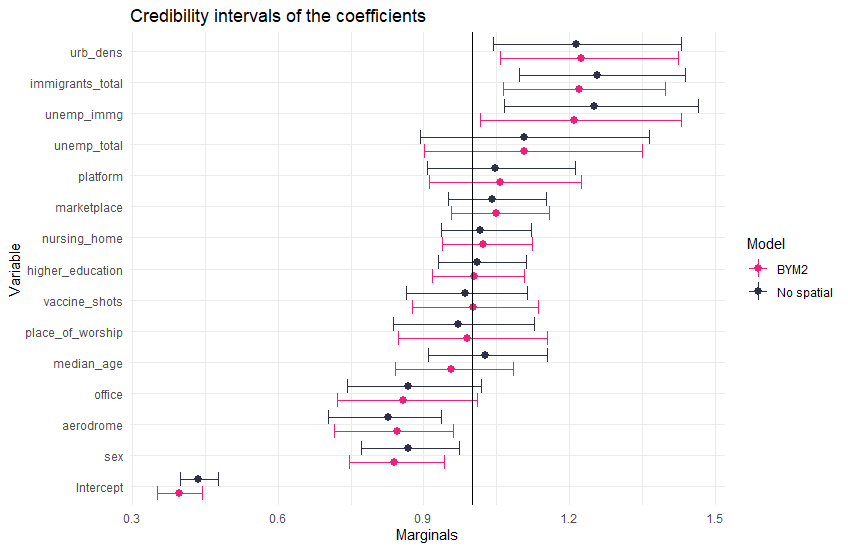
\includegraphics[width = \textwidth]{intervals_norway.png}
  \caption{The posterior mean and credibility intervals of the coefficients}
  \label{intervalNorway}
\end{figure}
The values of the coefficients and credibility intervals are shown in Table~\ref{fixedAllNorway_spatial}.
\begin{table}[H]
\caption{The fixed effects for the model. Values are rounded. A $^*$ denotes a significant effect. \label{fixedAllNorway_spatial}}
\begin{tabular}{l r r r r c}
\toprule
\textbf{Variable}	& \textbf{mean$_{\hbox{p}}$}	& \textbf{exp(mean$_{\hbox{p}}$)} & \textbf{exp(q0025$_{\hbox{p}}$)} & \textbf{exp(q0975$_{\hbox{p}}$)} & \textbf{sig.}\\
\midrule
(Intercept) & -0.895 & 0.409 & 0.368 & 0.454 & $^*$ \\
Total & \multirow{2}{*}{0.203}& \multirow{2}{*}{1.228}& \multirow{2}{*}{1.075}& \multirow{2}{*}{1.397}& \multirow{2}{*}{$^*$}\\
immigrants \\
Unemployed & \multirow{2}{*}{0.200} & \multirow{2}{*}{1.226} & \multirow{2}{*}{1.037} & \multirow{2}{*}{1.441} & \multirow{2}{*}{$^*$} \\
immigrants\\
Urban density & 0.180 & 1.201 & 1.042 & 1.393 & $^*$ \\
Vaccinations & 0.055 & 1.058 & 0.942 & 1.182\\
Platform & 0.049 & 1.053 & 0.912 & 1.213\\
Marketplace & 0.045 & 1.047 & 0.956 & 1.153 \\
Total & \multirow{2}{*}{0.044}& \multirow{2}{*}{1.050}& \multirow{2}{*}{0.863}& \multirow{2}{*}{1.267}\\
unemployment \\
Nursing & \multirow{2}{*}{0.012} & \multirow{2}{*}{1.013} & \multirow{2}{*}{0.931} & \multirow{2}{*}{1.109} \\
home\\
Higher & \multirow{2}{*}{-0.003}& \multirow{2}{*}{0.998}& \multirow{2}{*}{0.915}& \multirow{2}{*}{1.097}\\ 
education \\
Place of & \multirow{2}{*}{-0.018}& \multirow{2}{*}{0.985}& \multirow{2}{*}{0.849}& \multirow{2}{*}{1.142} \\
worship \\
Median age& -0.082 & 0.923 & 0.816 & 1.041 \\
Office & -0.138 & 0.874 & 0.742 & 1.026 \\
Sex & -0.211 & 0.811 & 0.723 & 0.906 & $^*$ \\
\bottomrule
\end{tabular}
\end{table}
For the hyperparameters, a value of 7.668 is reported for the precision and a value of 0.073 for $\phi$. Hence, 7.3\% of the marginal variance is explained by the structured effect. Therefore, this model is close to pure overdispersion.
\clearpage
\section{Choice of Hyperpriors}\label{sec:hyperprios}
As can be seen in Equation~\ref{pcprec}, there is flexibility when it comes to choosing the values for the standard deviation $\sigma_0$ as well as the probability $\alpha$. Therefore, an upper bound for the standard deviation can be chosen as well as the weight placed on this "tail event", describing how informative the resulting prior is. \\
Some of the issues that come with the choice of these hyperpriors were already discussed in Section~\ref{sec:issues}. \\
In the following, an assessment is made of how the performance of a Besag model, a BYM2 model and a Leroux model changes when playing around with the value for the standard deviation $\sigma_0$. To create these plots, models were calculated with $\sigma_0$ values of $\pmb{\sigma_0}=\left(0.1,0.11,0.12,...,5\right)$.\\
In Figure~\ref{comparison_norway_1} it can be seen that when choosing a higher value for $\sigma_0$, the DIC and WAIC is lower in the case of the Besag model and the BYM2 model. For the Leroux model, on the other hand, the WAIC gets lower until about 2 before it rises until around $\sigma_0 = 2.5$ and then flattens out. It is a positive sign that this is not the case with the BYM2 model, as it was designed to avoid exactly this kind of thing. \\
For the MAE in Figure~\ref{comparison_norway_2}, it can be seen that for all model types, a higher value for $\sigma_0$ leads to a lower MAE, however not by much.
\begin{figure}[H]
  \centering
  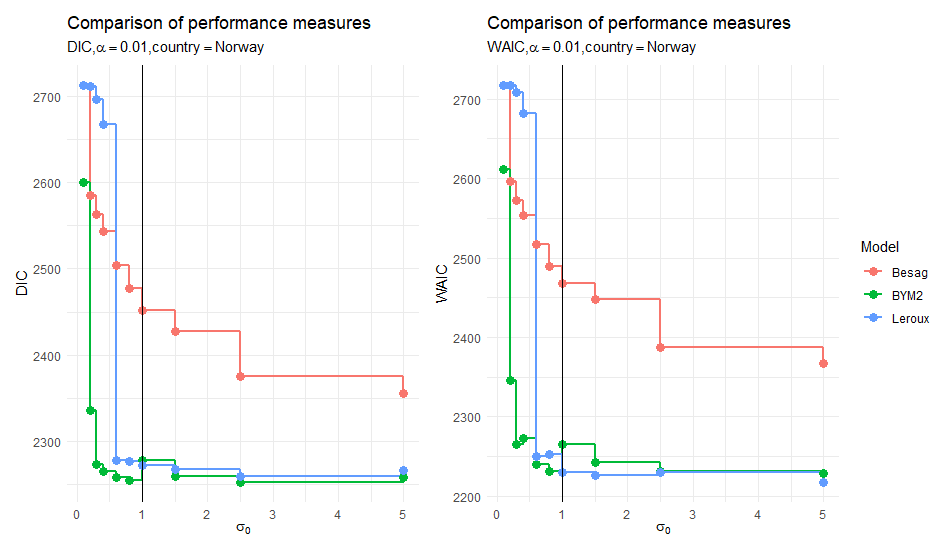
\includegraphics[width = \textwidth]{comparison_1_norway.png}
  \caption{Values of the DIC and the WAIC when changing the value for $\sigma_0$. The black line highlights the values for $\sigma_0$ = 1.}
  \label{comparison_norway_1}
\end{figure}
\begin{figure}[H]
  \centering
  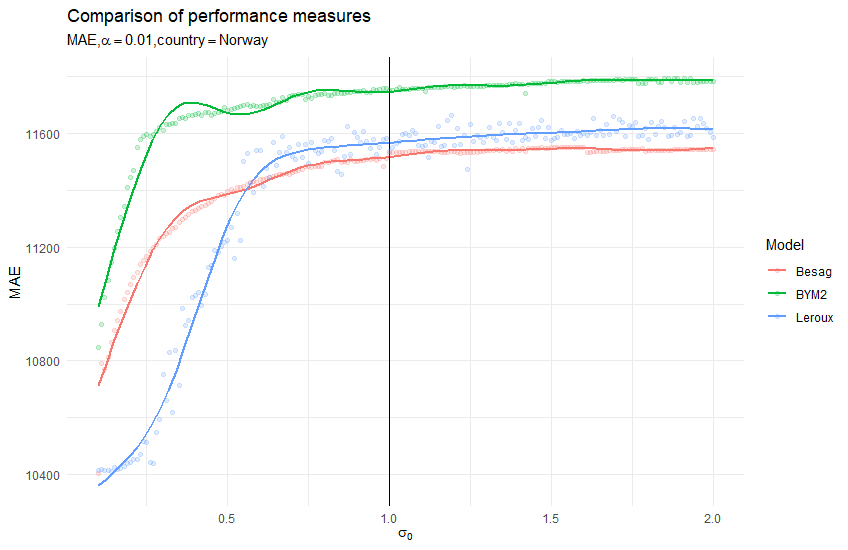
\includegraphics[width = \textwidth]{mae_norway.png}
  \caption{Value of the MAE when changing the value for $\sigma_0$. The black line highlights the values for $\sigma_0$ = 1.}
  \label{comparison_norway_2}
\end{figure}
By allowing the precision to be greater, the variance is forced to be smaller. Hence, choosing a lower value for the precision leads to lower values for the WAIC. While this indicates a better fit to the training data, Figure~\ref{comparison_norway_2} also shows that the MAE increases when a higher value for $\sigma_0$ is chosen, as the models overfit on the training data and therefore make worse predictions. \\
The corresponding figures for Germany are shown in Figure~\ref{comparison_germany_1} and Figure~\ref{comparison_germany_2} in the Appendix. \\
Figure~\ref{comparison_norway_5} shows how the credibility intervals of the coefficients of a BYM2 model change when the value for $\sigma_0$ is increased. The values of the coefficients tend to remain relatively similar most of the time, especially when the value of the coefficient is close to 1. However, a few times, for example for the variables immigrants\_total, platform and unemp\_immg, the values differ. Furthermore, the coefficients for $\sigma_0 = 1$ and $\sigma_0 = 2$ are more closer to 1 than the ones for $\sigma_0=0.1$.
\begin{figure}[H]
  \centering
  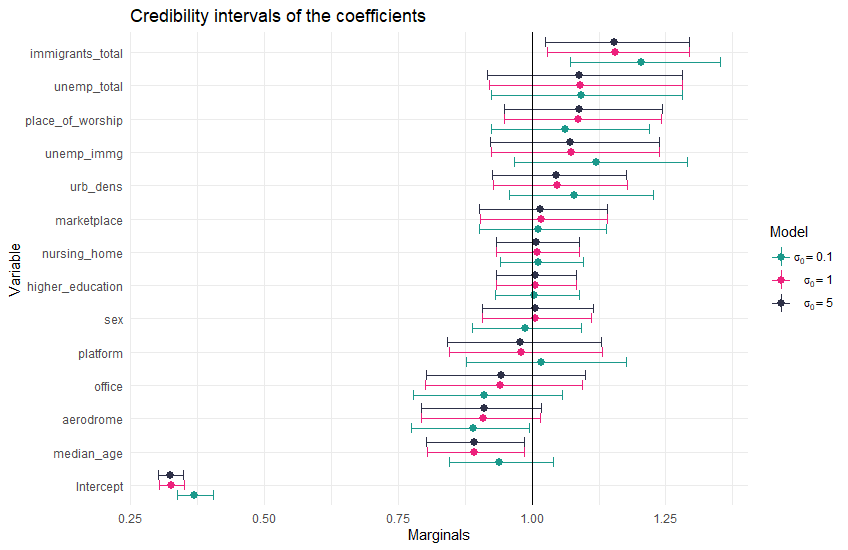
\includegraphics[width = \textwidth]{intervals_prior_norway.png}
  \caption{Comparison of the credibility intervals of a BYM2 model for different values of $\sigma_0$.}
  \label{comparison_norway_5}
\end{figure}
Having credibility intervals and posterior means that are very similar to each other, regardless of the value chosen for $\sigma_0$, is a great sign as it means that the calculated model is robust. That is, it means that the fixed covariates are important in their own right because they provide different information than the spatial field, even if the spatial field is allowed to be very smooth or coarse. This is exactly the case for Germany, which can be seen in Figure~\ref{comparison_germany_5}.
\begin{figure}[H]
    \centering
    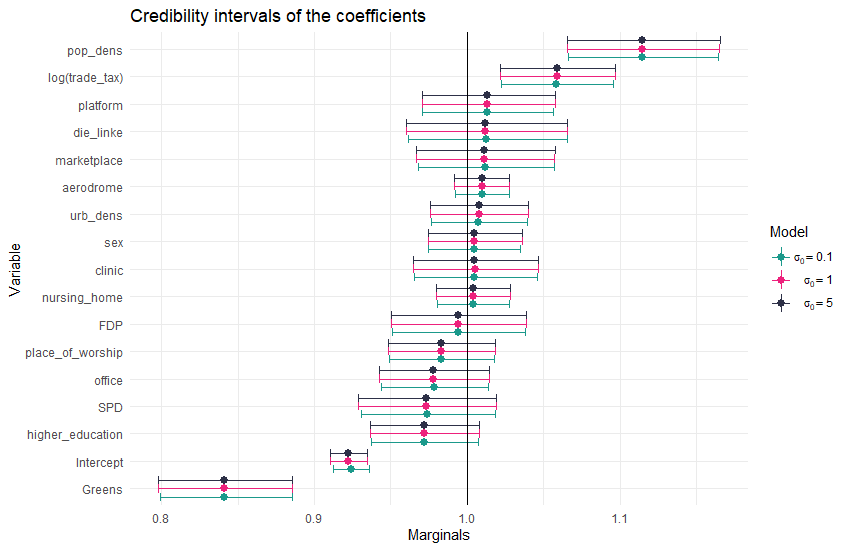
\includegraphics[width = \textwidth]{intervals_prior_germany.png}
    \caption{Comparison of the credibility intervals of a BYM2 model for different values of $\sigma_0$}
    \label{comparison_germany_5}
\end{figure}
Figure~\ref{comparison_norway_6} and Figure~\ref{comparison_norway_7} underline the problem of the models not being comparable with each other. Figure~\ref{comparison_norway_6} already shows huge differences in the spatial field of the Besag model and the Leroux model, with the spatial field of the Besag model looking smoother than the spatial field of the Leroux model. This is a sign that the Leroux model is quickly overfitting to the data.
In the left part of Figure~\ref{comparison_norway_7} the values of Equation~\ref{eq:bym2_1} are plotted, while in the right part the values of $u_{*}$ are plotted. \\
For the spatial field of the unstructured random effect, the values of the posterior mean are similar to the values of the Besag model. For the structured component, however, the absolute values are somewhat higher. Nevertheless, in both cases the values are far from the values for the Leroux model.
\begin{figure}[H]
  \centering
  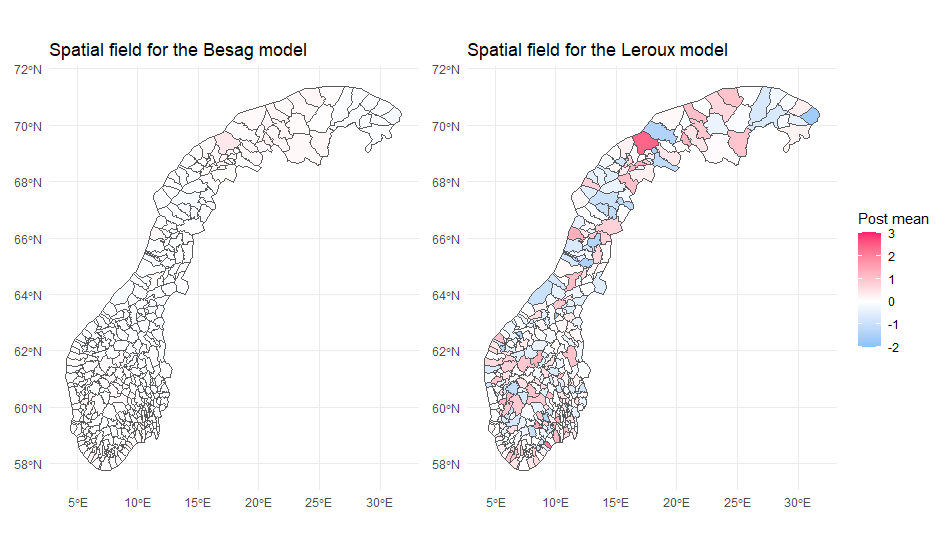
\includegraphics[width = \textwidth]{spatial_field_norway_1.png}
  \caption{Spatial field for a Besag model and a Leroux model.}
  \label{comparison_norway_6}
\end{figure}
\begin{figure}[H]
  \centering
  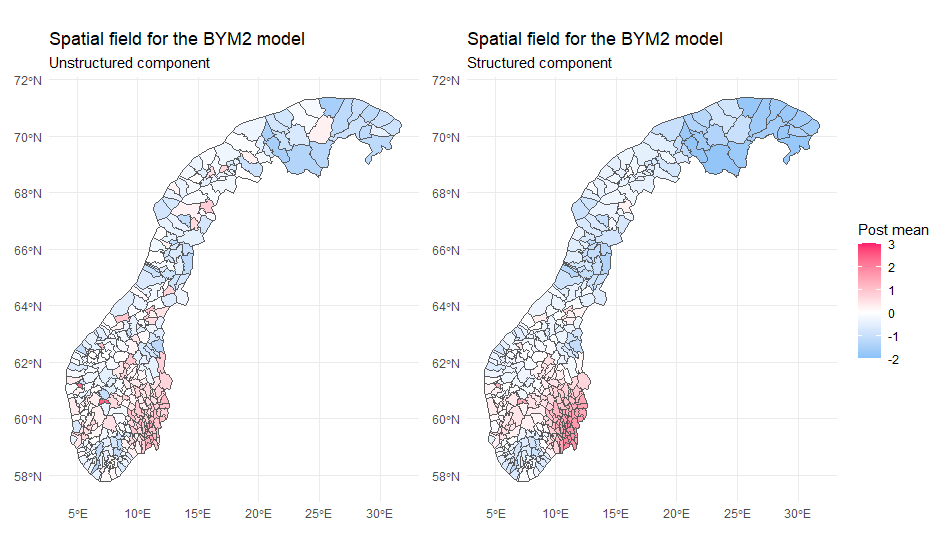
\includegraphics[width = \textwidth]{spatial_field_norway_2.png}
  \caption{Spatial fields for a BYM2 model.}
  \label{comparison_norway_7}
\end{figure}
The corresponding figures for Germany are shown in Figure~\ref{comparison_germany_6} and Figure~\ref{comparison_germany_7} in the Appendix. \\
Finally, looking at the spatial field of the structured component when changing the value for $\sigma_0$, as seen in Figure~\ref{comparison_norway_8}, it can be seen that for a small value like $\sigma_0 = 0.1$, the values of the posterior mean are mostly around 0, while for a higher value these values get slightly higher. The reason for this is simply that higher values for $\sigma_0$ make the spatial field fit the data more closely, making it less smooth.
\begin{figure}[H]
  \centering
  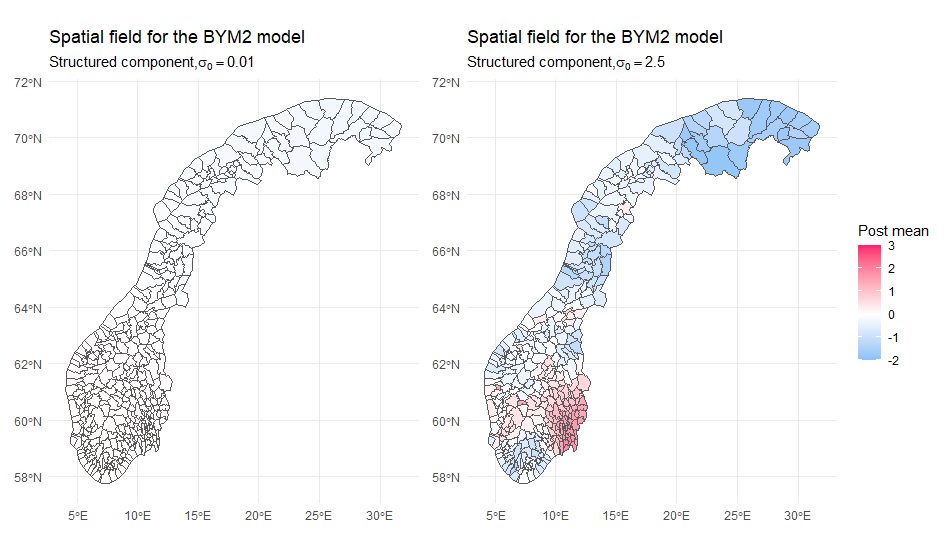
\includegraphics[width = \textwidth]{spatial_field_norway_3.png}
  \caption{Spatial fields for the structured component of a BYM2 model when changing the value for $\sigma_0$.}
  \label{comparison_norway_8}
\end{figure}
Looking at Figure~\ref{comparison_germany_8}, there are hardly any differences in the spatial fields for $\sigma_0=0,1$ and $\sigma_0=2$, which again shows how robust the model is for Germany.
\begin{figure}[H]
    \centering
    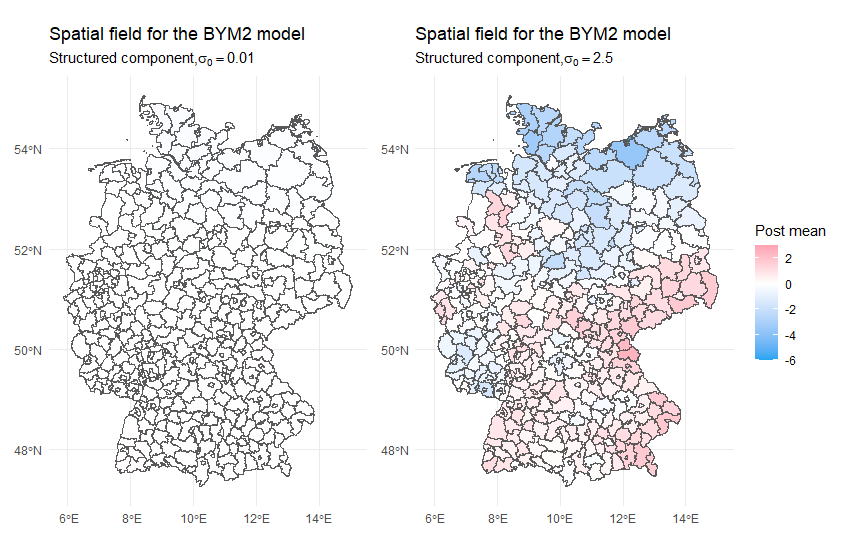
\includegraphics[width = \textwidth]{spatial_field_germany_3.png}
    \caption{Spatial fields for the structured component of a BYM2 model when changing the value for $\sigma_0$.}
    \label{comparison_germany_8}
\end{figure}

\clearpage
\section{Predictive models}
Another way to determine whether calculating a Bayesian spatial model is the right approach for this research question is to compare the calculated models with a completely different class of models, namely predictive models calculated using machine learning methods. The algorithms used in this chapter do not assume any kind of prior distributions or assumptions about the likelihood of the data.\\
The approach used to calculate these models is described in detail below.
\begin{itemize}
    \item[1.] Define the five base learners, which are:
    \begin{itemize}
        \item A regression tree
        \item A k-nearest neighbours (knn) algorithm
        \item A neural net
        \item A random forest
        \item An eXtreme Gradient Boosting (xGBoost) algorithm
    \end{itemize}
    \item[2.] Tune each algorithm using iterated F-Racing.
    \item[3.] Train each model using the parameters determined during the tuning process.
    \item[4.] Make predictions on the data.
\end{itemize}
The remainder of this chapter presents the results of the models calculated for Norway and Germany and provides some insights into how different factors influence infection rates. \\
I will add a small theory chapter on these models as well as the theory behind the interpretable ml stuff.
\subsection{Predictive models for Germany}
A look at Table~\ref{pred_perf} shows that the random forest had the lowest MAE of all the predictive models for both the training and test data, but still underperformed compared to the BYM2 model from Section~\ref{sec:spatial_germany}. In the remainder of this section, the random forest model is evaluated in more detail to gain an understanding of which variables influence infection rates according to the model.
\begin{table}[H] 
\caption{The MAE for the BYM2 model and the predictive models. \label{pred_perf}}
\begin{tabular}{l r r}
\toprule
\textbf{Model}	& \textbf{$\hbox{MAE}_{\hbox{train}}$} & \textbf{$\hbox{MAE}_{\hbox{test}}$}\\
\midrule
BYM2 & 103 & 1043\\
Regression tree & 2759 & 3249 \\
K-nearest neighbours & 1510 & 2430 \\
Neural net & 3942 & 4133 \\
Random forest & 1109 & 1895 \\
eXtreme Gradient Boosting & 1941 & 3036 \\
\bottomrule
\end{tabular}
\end{table}
Looking at the feature importance of the variables in Figure~\ref{importance_rf_germany}, it can be seen that log trade tax is the most important feature, followed by the number of clinics, platforms and marketplaces in a municipality. \\
Concept behind feature importance:  We measure the importance of a feature by calculating the increase in the model's prediction error after permuting the feature. A feature is "important" if shuffling its values increases the model error, because in this case the model relied on the feature for the prediction. A feature is "unimportant" if shuffling its values leaves the model error unchanged, because in this case the model ignored the feature for the prediction.
\begin{figure}[H]
  \centering
  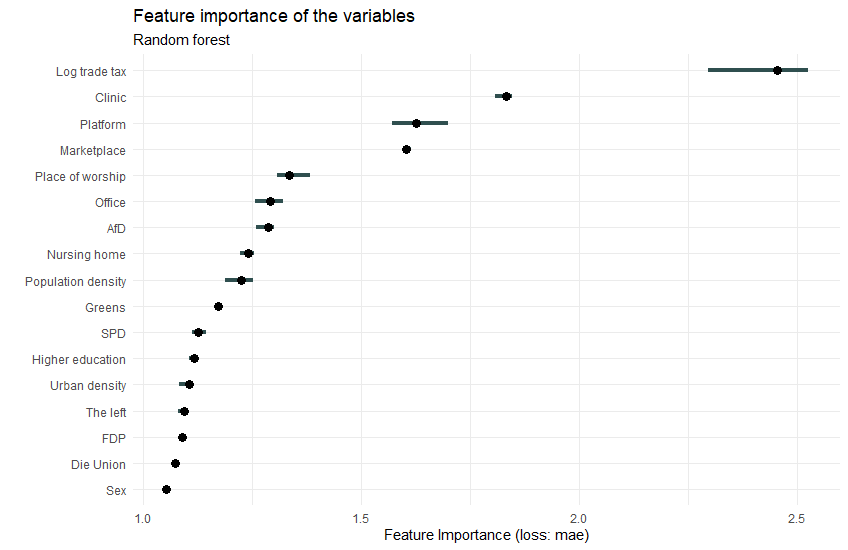
\includegraphics[width = \textwidth]{importance_rf_germany.png}
  \caption{The variable importance plots for the random forest.}
  \label{importance_rf_germany}
\end{figure}
To get a better idea of how the features influence the predicted outcome, the partial dependence plots for the two most important features are shown in Figure~\ref{pdp_rf_germany_1}, while Figure~\ref{pdp_rf_germany_3} shows how the two most important parties, the AfD and the Greens, influence the predicted outcome. For the logarithmic trade tax, a slow increase up until 0.5 can be seen before a steeper incline sets in, which eventually turns into a linear slope. For the number of clinic, it starts with a steep slope before changing to a less steep linear relationship and eventually flattening out. In general, however, the higher either value is, the higher the predicted outcome. Looking at the plots for the political parties, it can be seen that the higher the share of the vote for the AfD, the higher the predicted number of infections, while a higher share of the vote for the Greens leads to a lower predicted number of infections. The same relationship was observed in the BYM2 model, as can be seen in Table~\ref{FixedAllGermany_spatial}, but the effect for the Greens was not significant in this case. \\
Concept behind partial dependence plots:
The partial dependence plot (short PDP or PD plot) shows the marginal effect one or two features have on the predicted outcome of a machine learning model. A partial dependence plot can show whether the relationship between the target and a feature is linear, monotonic or more complex.
\begin{figure}[H]
  \centering
  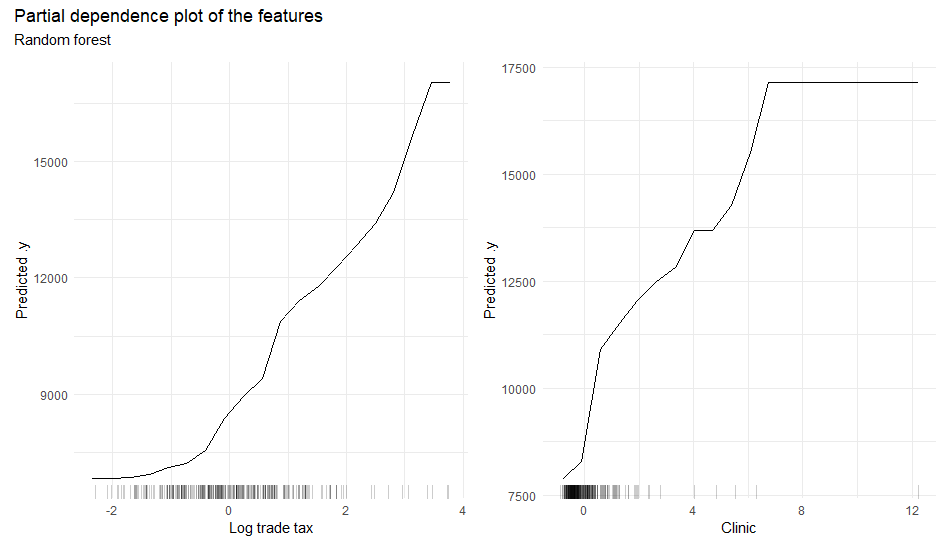
\includegraphics[width = \textwidth]{pdp_rf_germany_1.png}
  \caption{The partial dependence plots for the logarithmic trade tax and the number of clinics.}
  \label{pdp_rf_germany_1}
\end{figure}
\begin{figure}[H]
  \centering
  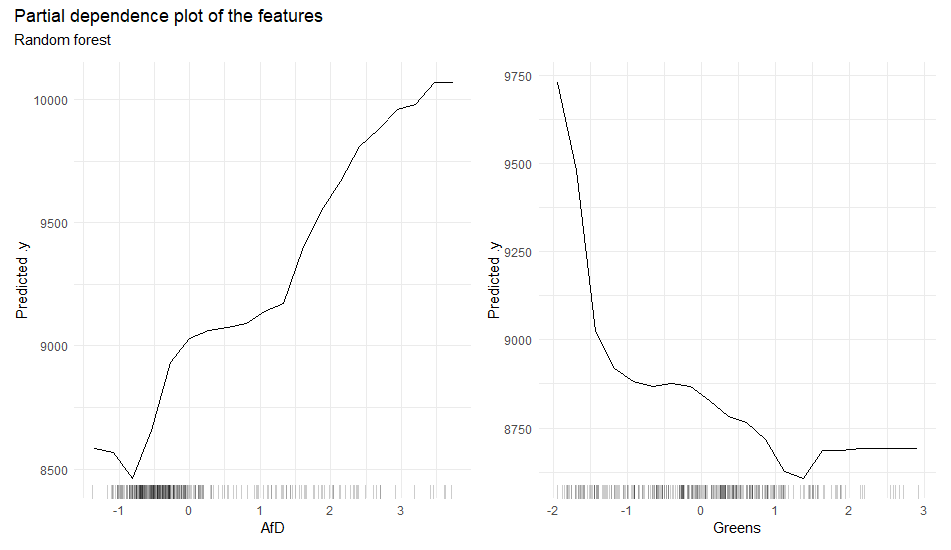
\includegraphics[width = \textwidth]{pdp_rf_germany_3.png}
  \caption{The partial dependence plots for the share of the vote the AfD and the Greens get.}
  \label{pdp_rf_germany_3}
\end{figure}
To check whether there are any interactions that could distort the relationship between the features shown in Figure~\ref{pdp_rf_germany_1} and Figure~\ref{pdp_rf_germany_3}, the ICE plots of these variables in Figure~\ref{ice_rf_germany_1} and Figure~\ref{ice_rf_germany_3} can be looked at. All curves seem to follow the same course, so there are no obvious interactions. This means that the PDP already represents a good summary of the relationships between the displayed features and the predicted number of infections. \\
Concept behind ice curves: Individual Conditional Expectation (ICE) plots display one line per instance that shows how the instance's prediction changes when a feature changes. The partial dependence plot for the average effect of a feature is a global method because it does not focus on specific instances, but on an overall average. The equivalent to a PDP for individual data instances is called individual conditional expectation (ICE) plot. What is the point of looking at individual expectations instead of partial dependencies? Partial dependence plots can obscure a heterogeneous relationship created by interactions.
\begin{figure}[H]
  \centering
  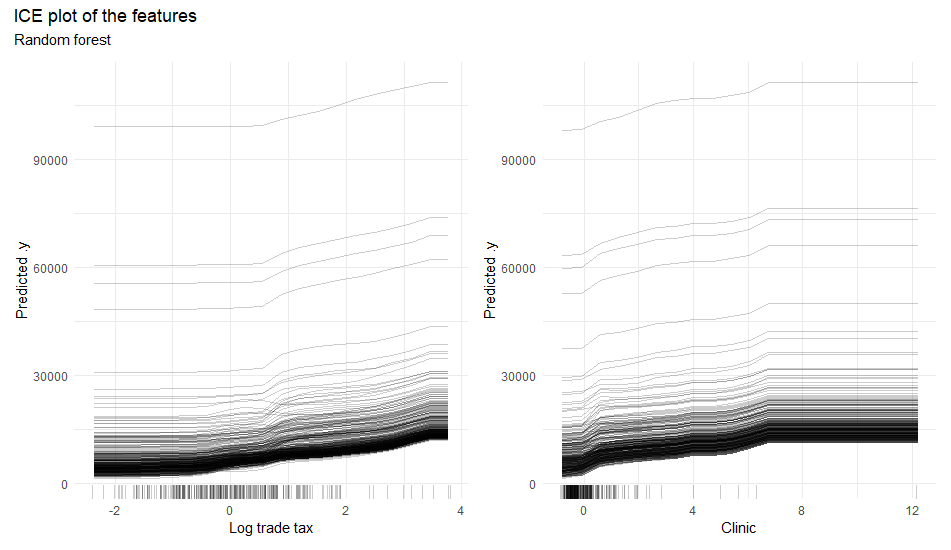
\includegraphics[width = \textwidth]{ice_rf_germany_1.png}
  \caption{The individual conditional expectation for the logarithmic trade tax and the number of clinics.}
  \label{ice_rf_germany_1}
\end{figure}
\begin{figure}[H]
  \centering
  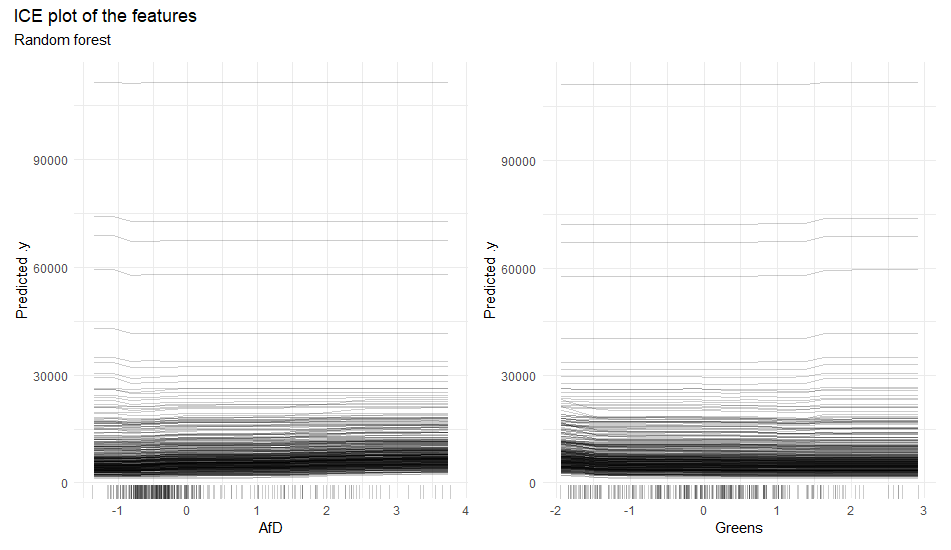
\includegraphics[width = \textwidth]{ice_rf_germany_3.png}
  \caption{The individual conditional expectation for the share of the vote the AfD and the Greens get.}
  \label{ice_rf_germany_3}
\end{figure}
Lastly, looking at the Shapley values for the region of Hannover in Figure~\ref{shapley_rf_germany}, the prediction is nearly 50,000 above the average prediction. The number of marketplaces in the region increased the prediction the most, followed by the logarithmic trade tax and the number of offices in the region. For the city of Munich it was the same three features, however this time the logarithmic trade tax increased the prediction the most, followed by the number of offices and the number of marketplaces. For Munich, the actual prediction was around 33,000 above the average prediction. \\
Concept behind the shapley value: The Shapley value of a feature value is not the difference of the predicted value after removing the feature from the model training. The interpretation of the Shapley value is: Given the current set of feature values, the contribution of a feature value to the difference between the actual prediction and the mean prediction is the estimated Shapley value.
\begin{figure}[H]
  \centering
  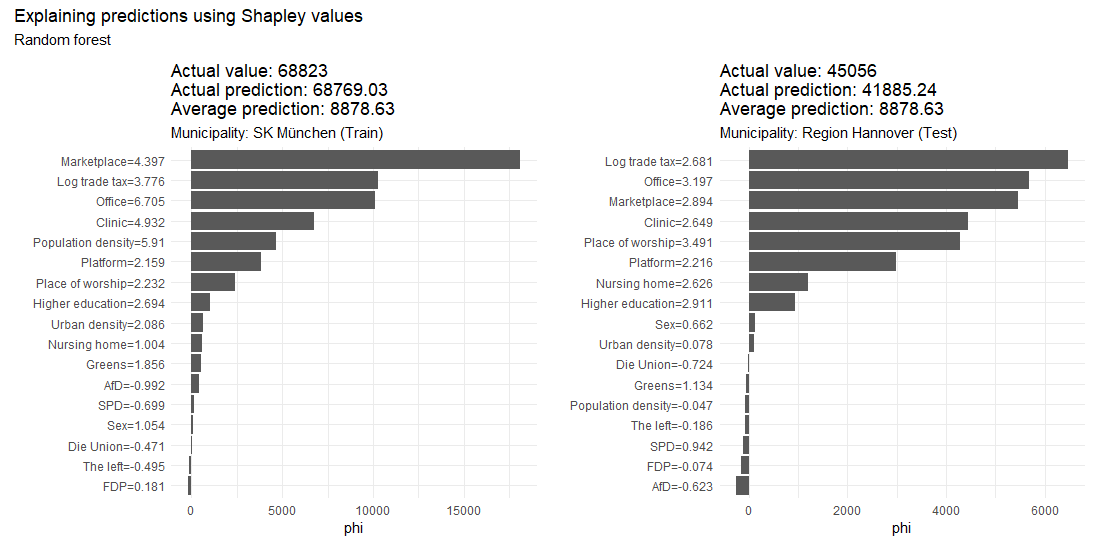
\includegraphics[width = \textwidth]{shapley_rf_germany.png}
  \caption{Shapley values for the cities of Munich and Hannover.}
  \label{shapley_rf_germany}
\end{figure}
%https://christophm.github.io/interpretable-ml-book/pdp.html
\subsection{Predictive models for Norway}
Looking at the performance of the different algorithms in Table~\ref{pred_perf_norway}, again, the random forest model had the lowest MAE of all the predictive models for the training and test data, but performed worse than the BYM2 model from Section~\ref{sec:spatial_norway}. Therefore, the random forest model is again evaluated in more detail to gain an understanding of which variables influence the infection rates according to the model.
\begin{table}[H] 
\caption{The MAE for the BYM2 model and the predictive models. \label{pred_perf_norway}}
\begin{tabular}{l r r}
\toprule
\textbf{Model}	& \textbf{$\hbox{MAE}_{\hbox{train}}$} & \textbf{$\hbox{MAE}_{\hbox{test}}$}\\
\midrule
BYM2 & 160 & 89\\
Regression tree & 399 & 279 \\
K-nearest neighbours & 184 & 148 \\
Neural net & 392 & 297 \\
Random forest & 161 & 134 \\
eXtreme Gradient Boosting & 251 & 196 \\
\bottomrule
\end{tabular}
\end{table}
Looking at the feature importance of the variables in Figure~\ref{importance_rf_norway}, the most important feature is the number of places of worship in a municipality, followed by the number of offices and the number of public transport platform. \\
\begin{figure}[H]
  \centering
  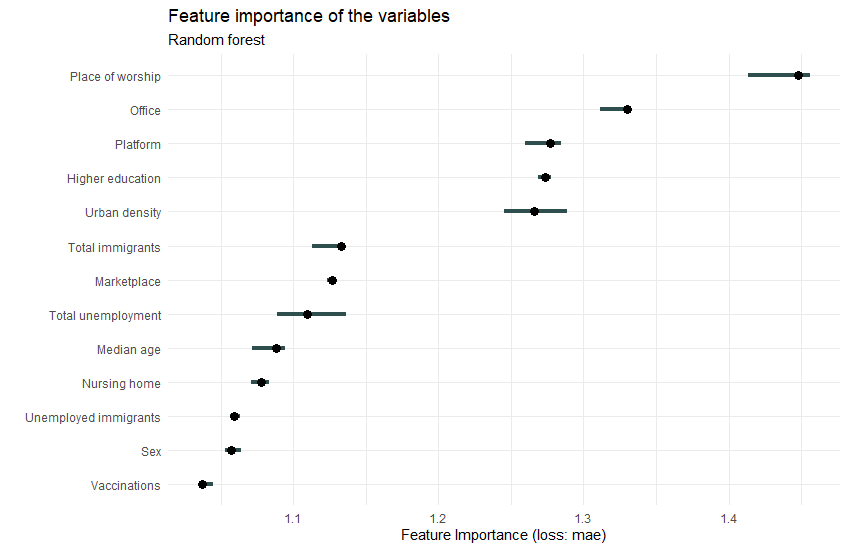
\includegraphics[width = \textwidth]{importance_rf_norway.png}
  \caption{The variable importance plots for the random forest.}
  \label{importance_rf_norway}
\end{figure}
Figure~\ref{pdp_rf_norway_1} shows how the predicted number of infections changes as the number of places of worship and offices in a community increases. For places of worship, a slow increase is seen until 3, followed by a steep increase that continues until 7 and then ends in a plateau. For the number of offices, it is a slow increase until about 2.5, followed by a steep increase until about 6 before ending on a plateau.
\begin{figure}[H]
  \centering
  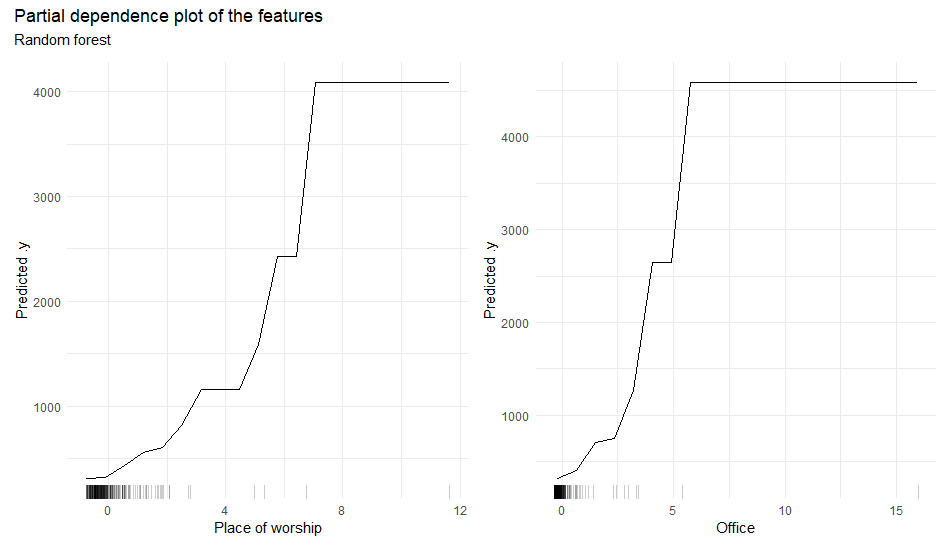
\includegraphics[width = \textwidth]{pdp_rf_norway_1.png}
  \caption{The partial dependence plots for the number of places of worship and the number of offices.}
  \label{pdp_rf_norway_1}
\end{figure}
The curves display in the ICE plot in Figure~\ref{pdp_rf_norway_1} all follow the same course, so there are no obvious interactions. Therefore, again, the PDP already represents a good summary of the relationships between the displayed features and the predicted number of infections. \\
\begin{figure}[H]
  \centering
  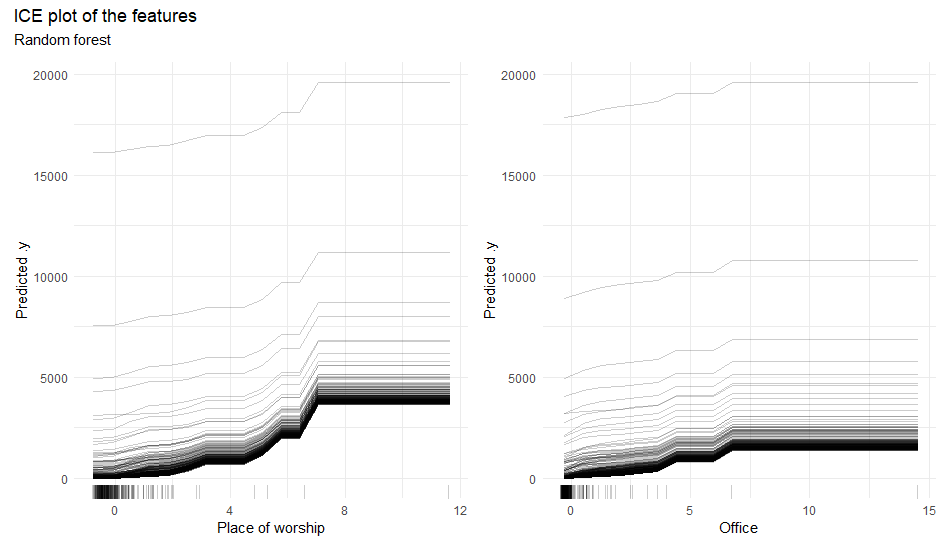
\includegraphics[width = \textwidth]{ice_rf_norway_1.png}
  \caption{The individual conditional expectation for the logarithmic trade tax and the number of clinics.}
  \label{ice_rf_norway_1}
\end{figure}
Finally, looking at the Shapley values for Tromsø municipality in Figure~\ref{shapley_rf_norway}, the prediction is about 1,100 above the average prediction. The feature that increases the prediction the most is the number of nursing homes in the municipality, while the number of marketplaces is the feature that decreases the prediction the most.
For Nordre Follo, the prediction is about 1,000 above the average prediction, with the number of public transport platforms and urban density being the two features that increase the prediction the most, while the number of offices and higher educational buildings are the feature that decrease the prediction the most.
\begin{figure}[H]
  \centering
  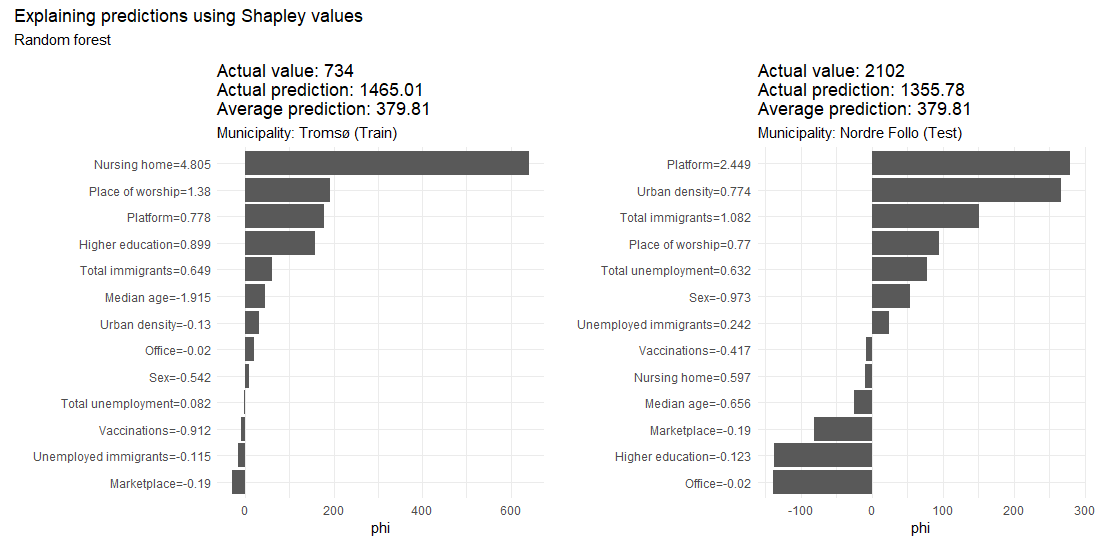
\includegraphics[width = \textwidth]{shapley_rf_norway.png}
  \caption{Shapley values for the municipalties of Tromsø and Nordre Follo.}
  \label{shapley_rf_norway}
\end{figure}
\clearpage
\section{Temporal models}
I will write some kind of introduction here relating to temporal effects such as government measures or waves of covid. i will also write sth about baseline temporal models used for comparison
\subsection{Choice of Likelihood}
As with the non-temporal models calculated in Section~\ref{sec:nospatial} and Section~\ref{ch:spatial}, a probability must first be found that describes the distribution of the daily number of infections in each country. Returning to the Cullen and Frey graph, Figure~\ref{cf_germany_ts} and Figure~\ref{cf_norway_ts} show that the observations do not actually follow a normal, negative binomial or Poisson distribution.
\begin{figure}[H]
  \centering
  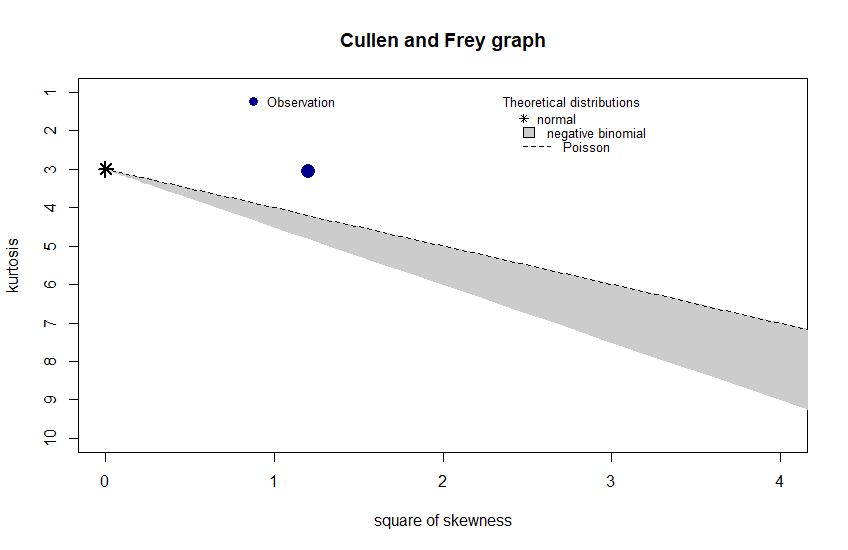
\includegraphics[width = 0.8\textwidth]{cf_germany_ts.png}
  \caption{The Cullen and Frey graph for Germany}
  \label{cf_germany_ts}
\end{figure}
\begin{figure}[H]
  \centering
  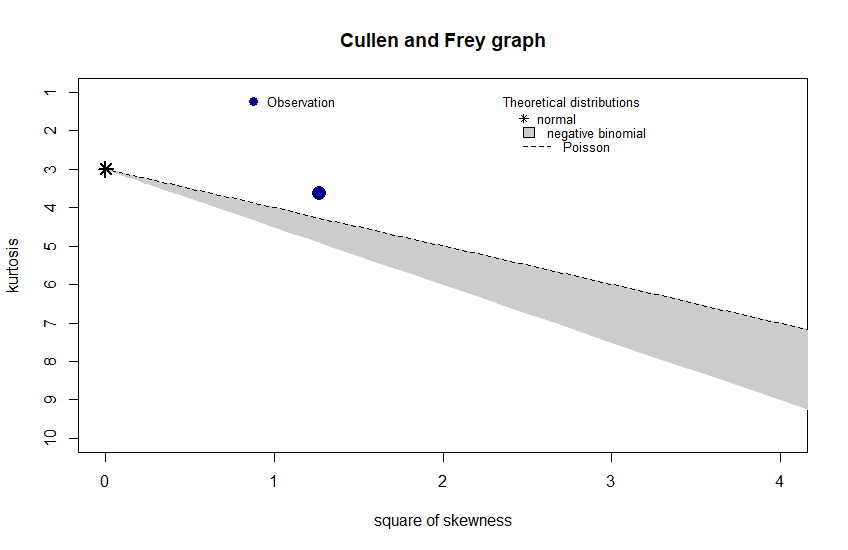
\includegraphics[width = 0.8\textwidth]{cf_norway_ts.png}
  \caption{The Cullen and Frey graph for Norway}
  \label{cf_norway_ts}
\end{figure}
After fitting all three distributions to the data using the maximum likelihood method, QQ-plots and the empirical and theoretical cumulative density function can be used to help decide which likelihood to choose. The QQ-plots in Figure~\ref{fitNegbinomGermany_ts} and Figure~\ref{fitNormalGermany_ts} clearly show that there is no linear relationship between the theoretical quantiles and the sample quantiles for both distributions, while the empirical CDF roughly follows the theoretical CDF in both cases. The plots for the Poisson distribution as well as all plots for the Norwegian municipalities are in Section~\ref{sec:temp_fit_germany} and section~\ref{sec:temp_fit_norway} in the Appendix.
\begin{figure}[H]
  \centering
  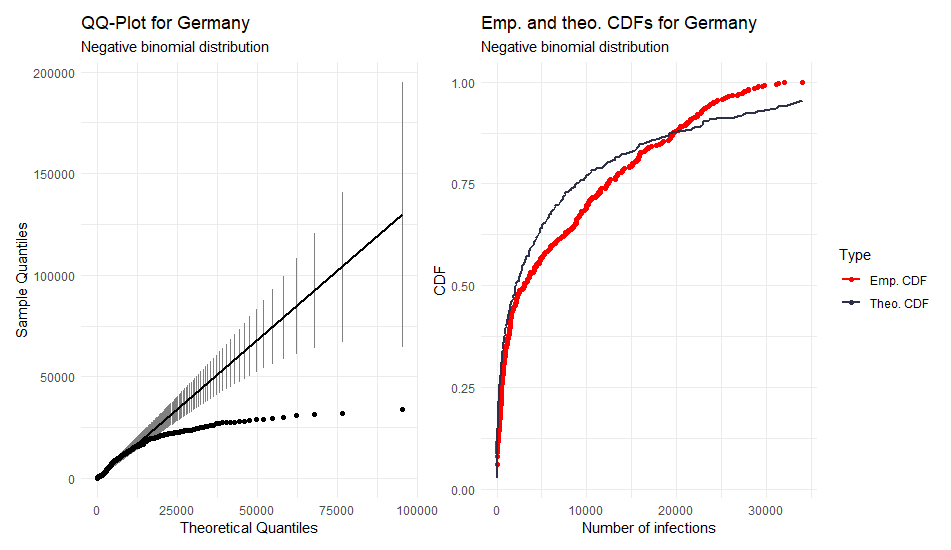
\includegraphics[width = 0.8\textwidth]{fit_nbinom_germany_ts.png}
  \caption{A negative binomial fit to the number of cases in German municipalities}
  \label{fitNegbinomGermany_ts}
\end{figure}
\begin{figure}[H]
  \centering
  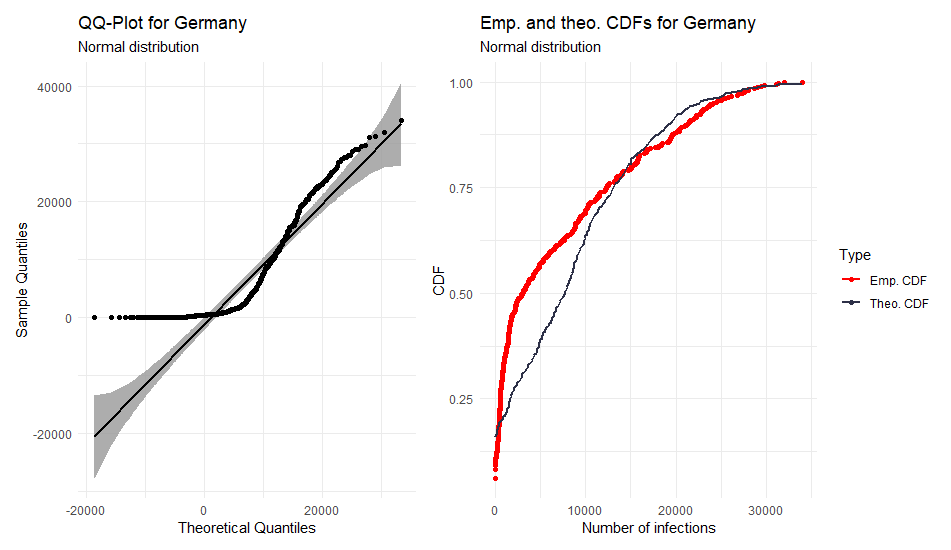
\includegraphics[width = 0.8\textwidth]{fit_normal_germany_ts.png}
  \caption{A normal fit to the number of cases in German municipalities}
  \label{fitNormalGermany_ts}
\end{figure}
Looking at the AIC for all the distribution fits shown in Table~\ref{aic_temporal}, the negative binomial distribution again seems to be the best fit for the data. For Germany the mean and standard deviation are 7274 and 8429 respectively, while for Norway these moments are 256 and 266. This again explains the poor fit of the Poisson distribution, since an equal mean and variance are assumed for the Poisson distribution.
\begin{table}[H] 
\caption{The AIC for different distributions for Germany and Norway \label{aic_temporal}}
\begin{tabular}{l l r}
\toprule
\textbf{Country}	& \textbf{Distribution}	& \textbf{AIC} \\
\midrule
Germany & Normal & 10461 \\
Germany & Poisson & 4762604 \\
Germany & Negative Binomial & 9462 \\
Norway & Normal & 6600 \\
Norway & Poisson & 131469 \\
Norway & Negative Binomial & 6076 \\
\bottomrule
\end{tabular}
\end{table}
Overlaying the number of infections with a negative binomial distribution and a normal distribution using the estimated parameters, as shown in Figure~\ref{fitDistrGermany_ts}, reinforces the assumption of the negative binomial distribution, which is then used as the assumed probability of the data for the models calculated in this chapter. The graph for Norway can be seen in Figure~\ref{fitDistrNorway_ts}.
\begin{figure}[H]
  \centering
  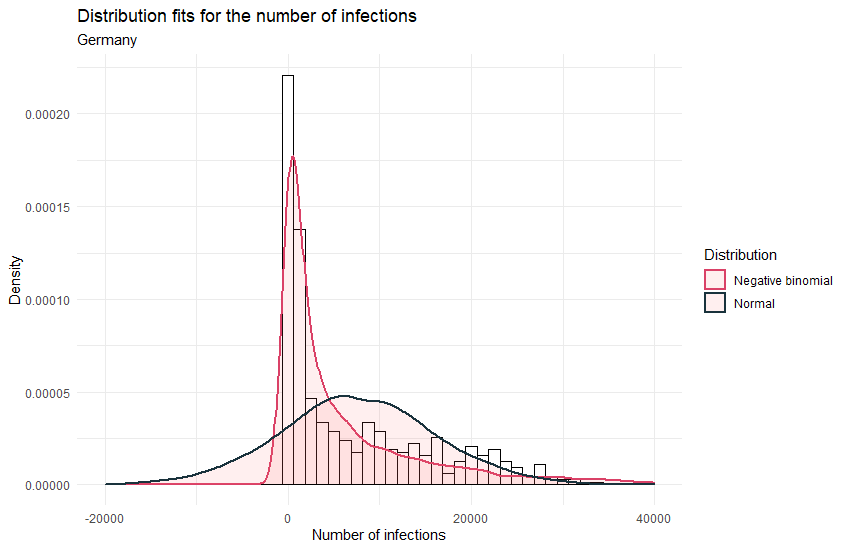
\includegraphics[width = 0.8\textwidth]{distrfit_germany_ts.png}  
  \caption{Histogram for the number of cases in German municipalities with a normal and a negative binomial distribution overlayed.}
  \label{fitDistrGermany_ts}
\end{figure}
\clearpage
\subsection{Temporal models for Germany}
For Germany, 502 data points are available, starting on 7 January 2020 and ending on 22 May 2021. Of these 502 data points, the first 482 are used for model training, while the last 20 are used for the analysis. Due to the temporal effect, a random split would not make sense as this may lead to a look-ahead bias as the model would use information that was not yet known or available during the analysed period. After removing variables using the VIF method already used for the non-temporal models, the trained model used the following variables:
\begin{itemize}
    \item Measures taken in relation to contact tracing.
    \item Measures taken in relation to restrictions on internal movement.
    \item Measures taken in relation to the use of face masks.
    \item Measures taken in relation to the requirement to remain at home.
    \item The mobility at workplaces.
    \item The season of the year.
    \item The relative frequency of the main strain of Covid-19.
    \item The relative frequency of variant 20E.
    \item The relative abundance of variant 20L, also known as B.1.1.7
\end{itemize}
A second-order random walk is chosen for the temporal effect. The performance measures of this model and the temporal baseline models are shown in Table~\ref{germany_temporal}. While the AR(1) process has by far the lowest MAE in training, it has the second highest MAE in testing. The temporal model, besides the AR(1), has the lowest MAE during training and the overall lowest MAE during testing, indicating that the model fits the data best.
\begin{table}[H] 
\caption{The performance measures for different types of temporal models for Germany. \label{germany_temporal}}
\begin{tabular}{l r r r r r}
\toprule
\textbf{Model}	& \textbf{DIC}	& \textbf{WAIC} & \textbf{CPO} & \textbf{$\hbox{MAE}_{\hbox{train}}$} & \textbf{$\hbox{MAE}_{\hbox{test}}$}\ \\
\midrule
Only date as covariate & 8815 & 8816 & -4408 & 4915 & 27450 \\
Random walk of second order & 7522 & 7519 & -3760 & 2009 & 6180 \\
AR(1) process & 5950 & 5924 & -3877 & 18 & 7524 \\
Temporal model &  7524 & 7521 & -3777 & 1931 & 5821 \\
\bottomrule
\end{tabular}
\end{table}
Looking at the predicted number of infections from the temporal model in Figure~\ref{predictions_1_germany}, it can be seen that the predictions for the training data follow roughly the same path as the actual numbers, as three waves can be clearly seen. For the test data depicted more clearly in Figure~\ref{predictions_2_germany}, the predicted number of cases shows a very slow increase and it can also be seen that the "weekend effect", which means that fewer infections are reported on the weekend, has not been captured. Furthermore, the more recent a data point is in the test set, the greater the uncertainty associated with the prediction.
\begin{figure}[H]
  \centering
  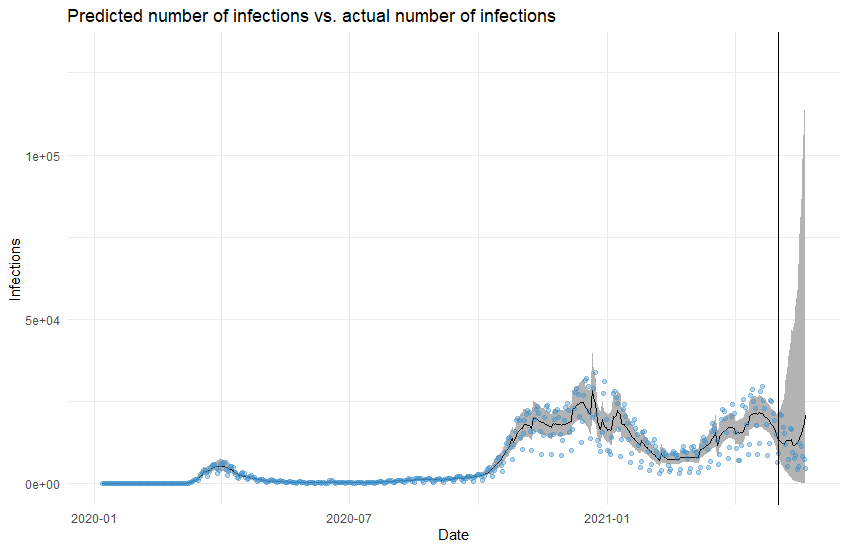
\includegraphics[width = 0.8\textwidth]{predictions_1_germany.png}
  \caption{The predicted number of infections in Germany according to the temporal model. The vertical line indicates where the test data begins.}
  \label{predictions_1_germany}
\end{figure}
\begin{figure}[H]
  \centering
  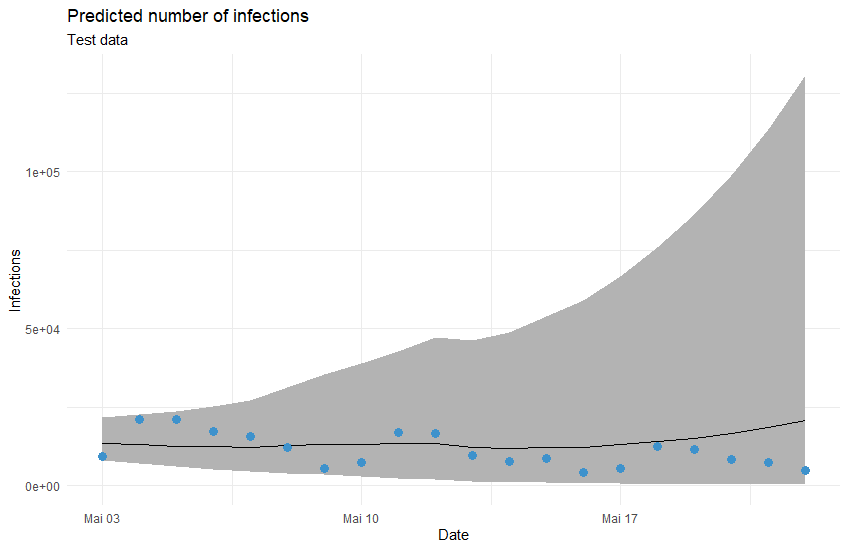
\includegraphics[width = 0.8\textwidth]{predictions_2_germany.png}
  \caption{The predicted number of infections in Germany according to the temporal model.}
  \label{predictions_2_germany}
\end{figure}
Another way to look at the predictions is to compare the 7-day incidence of the actual number of infections and the predicted number of infections, as daily variations such as the "weekend effect" should be smoothed out. Figure~\ref{incidence_germany} shows that the predicted 7-day incidence again follows the actual data very well, even a little for the test data. However, this is because for the first few days of test data, the incidence depends on the predicted number of infections for a few days of training data. Once it is only test data, the 7-day decline slowly stops before a steep slope starts, in contrast to the actual 7-day incidence, which is still falling.
\begin{figure}[H]
  \centering
  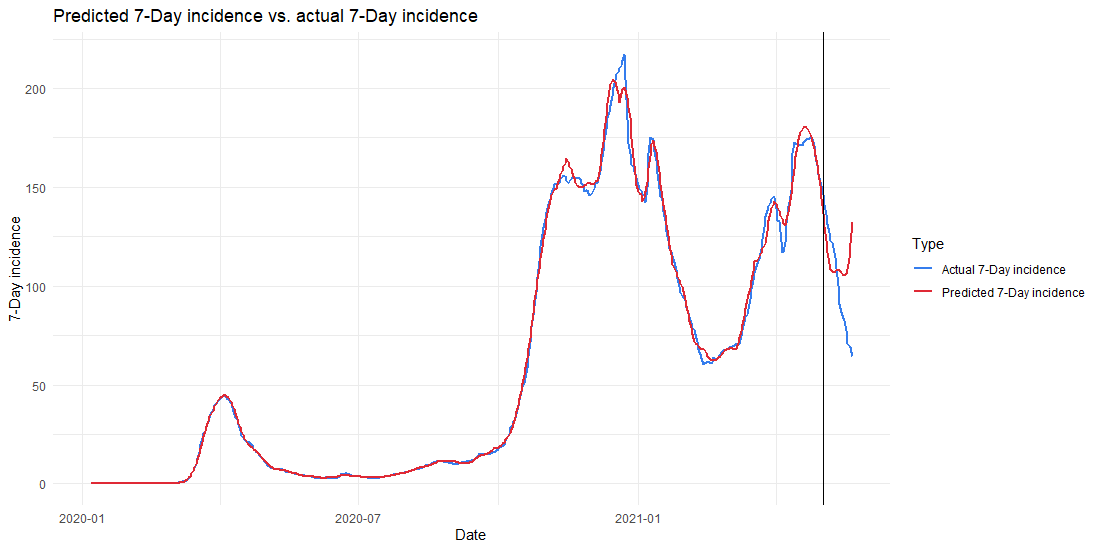
\includegraphics[width = 0.8\textwidth]{incidence_germany.png}  
  \caption{The 7-day incidence of the actual number of infections and the predicted number of infections. The vertical line indicates where the test data begins.}
  \label{incidence_germany}
\end{figure}
Looking at the posterior temporal trend for Germany in Figure~\ref{trend_germany}, the first two waves are clearly visible, with the second wave having two peaks, the first in early November 2020 and the second in mid-December 2020. The peak of the first and third waves is in late March 2020 and mid-April 2021, respectively. After the third peak, a steep increase sets in, as with the 7-day incidence in Figure~\ref{incidence_germany}, which is clearly not the case when looking at the actual data.
\begin{figure}[H]
  \centering
  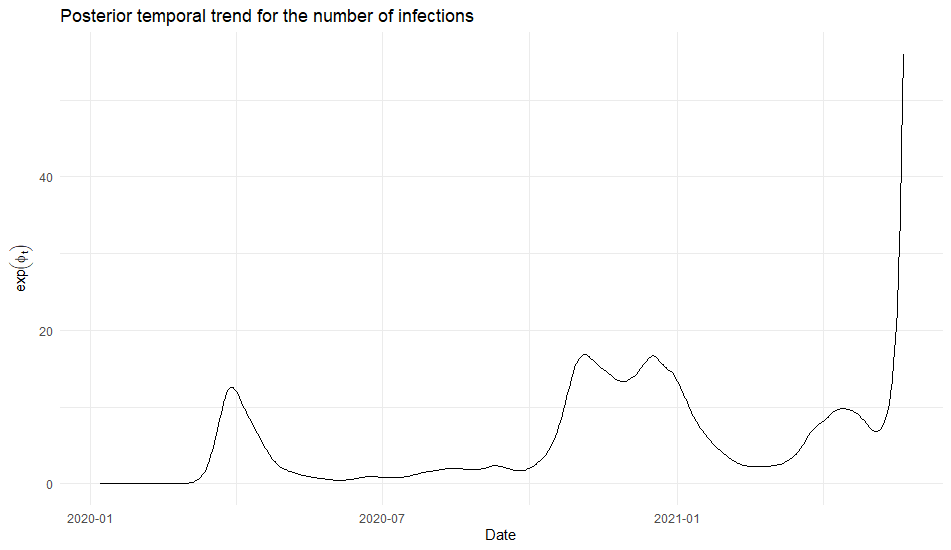
\includegraphics[width = 0.8\textwidth]{temp_trend_germany.png}  
  \caption{The posterior temporal trend for the number of infections.}
  \label{trend_germany}
\end{figure}
The covariates of the model are presented in Table~\ref{fixed_germany_temporal}. Apart from the intercept, the only significant effect is the mobility at workplaces.
\begin{table}[H]
\caption{The fixed effects for the model. Values are rounded. A $^*$ denotes a significant effect. \label{fixed_germany_temporal}}
\begin{tabular}{l r r r r c}
\toprule
\textbf{Variable}	& \textbf{mean$_{\hbox{p}}$}	& \textbf{exp(mean$_{\hbox{p}}$)} & \textbf{exp(q0025$_{\hbox{p}}$)} & \textbf{exp(q0975$_{\hbox{p}}$)} & \textbf{sig.}\\
\midrule
(Intercept) & -1.592 & 0.228 & 0.079 & 0.518 & $^*$ \\
Variant 20L & 0.658 & 2.117 & 0.836 & 4.476 \\
Variant 20E & 0.320 & 1.407 & 0.926 & 2.059 \\
Restrictions internal & \multirow{3}{*}{0.235} & \multirow{3}{*}{1.298} & \multirow{3}{*}{0.813} & \multirow{3}{*}{1.970} \\
movement \\
Movement restricted \\
Workplace mobility & 0.168 & 1.186 & 1.029 & 1.359 & $^*$\\
Season winter & 0.112 & 1.161 & 0.653 & 1.918 \\
Season spring & 0.034 & 1.082 & 0.574 & 1.858 \\
Stay home & \multirow{3}{*}{0.022} & \multirow{3}{*}{1.044} & \multirow{3}{*}{0.687} & \multirow{3}{*}{1.517} \\
requirements \\
Recommended \\
Facial coverings & \multirow{2}{*}{0.018} & \multirow{2}{*}{1.070} & \multirow{2}{*}{0.551} & \multirow{2}{*}{1.884} \\
Recommended \\
Facial coverings & \multirow{3}{*}{-0.008} & \multirow{3}{*}{1.109} & \multirow{3}{*}{0.398} & \multirow{3}{*}{2.506} \\
Required in some \\ 
public spaces \\
Stay home & \multirow{3}{*}{-0.014} & \multirow{3}{*}{1.009} & \multirow{3}{*}{0.650} & \multirow{3}{*}{1.492}\\
requirements \\
Required (exc. essent.) \\
Restrictions internal & \multirow{3}{*}{-0.021} & \multirow{3}{*}{1.004} & \multirow{3}{*}{0.632}& \multirow{3}{*}{1.522} \\
movement \\
Recommended \\
Contact tracing & \multirow{2}{*}{-0.047} & \multirow{2}{*}{0.976} & \multirow{2}{*}{0.630} & \multirow{2}{*}{1.454} \\
Limited tracing \\
Main variant & -0.134 & 0.920 & 0.470 & 1.622 \\
Season summer & -0.341 & 0.739 & 0.412 & 1.216 \\
Contact tracing & \multirow{2}{*}{-2.095} & \multirow{2}{*}{0.228} & \multirow{2}{*}{0.010} & \multirow{2}{*}{1.035} \\
No tracing \\
\bottomrule
\end{tabular}
\end{table}
\subsection{Temporal models for Norway}
For Norway, 473 data points are available, starting on 5 February 2020 and ending on 22 May 2021. Of these 473 data points, the first 453 are used for model training, while the last 20 are used for the analysis. After the removal of some variables, the following features remained:
\begin{itemize}
    \item Measures taken in relation to restrictions on internal movement.
    \item Measures taken in relation to the requirement to remain at home.
    \item The mobility at workplaces.
    \item The mobility at groceries and pharmacies.
    \item The season of the year.
    \item The relative frequency of the main strain of Covid-19.
    \item The relative frequency of variant 20E.
    \item The relative abundance of variant 20L, also known as B.1.1.7
\end{itemize}
Again, a second-order random walk is chosen for the temporal effect. The performance measures of this model and the temporal baseline models are shown in Table~\ref{norway_temporal}. The lowest MAE during training was again observed for the AR(1) process, followed by the temporal model and the second-order random walk. The temporal model then showed the best performance in terms of MAE for the test set, followed by the second-order random walk and the AR(1) process.
\begin{table}[H] 
\caption{The performance measures for different types of temporal models for Norway. \label{norway_temporal}}
\begin{tabular}{l r r r r r}
\toprule
\textbf{Model}	& \textbf{DIC}	& \textbf{WAIC} & \textbf{CPO} & \textbf{$\hbox{MAE}_{\hbox{train}}$} & \textbf{$\hbox{MAE}_{\hbox{test}}$}\ \\
\midrule
Only date as covariate & 5567 & 5568 & -2784 & 130 & 446 \\
Random walk of second order & 4603 & 4603 & -2387 & 55 & 119 \\
AR(1) process & 4602 & 4599 & -2315 & 38 & 110 \\
Temporal model &  4613 & 4613 & -2432 & 53 & 100 \\
\bottomrule
\end{tabular}
\end{table}
For the predicted number of infections shown in Figure~\ref{predictions_1_norway}, 4 peaks are seen for the training data, just like for the actual data. The rest of the predicted infection numbers also follow the actual infection numbers very closely, which is not too surprising given the low MAE shown in Table~\ref{norway_temporal}. For the test data shown in Figure~\ref{predictions_2_norway}, it is very similar to the graph for Germany in Figure~\ref{predictions_2_germany}, as the "weekend effect" is not captured, a slow increase in the predicted infection numbers can be seen, as well as an increasing uncertainty in the predictions.
\begin{figure}[H]
  \centering
  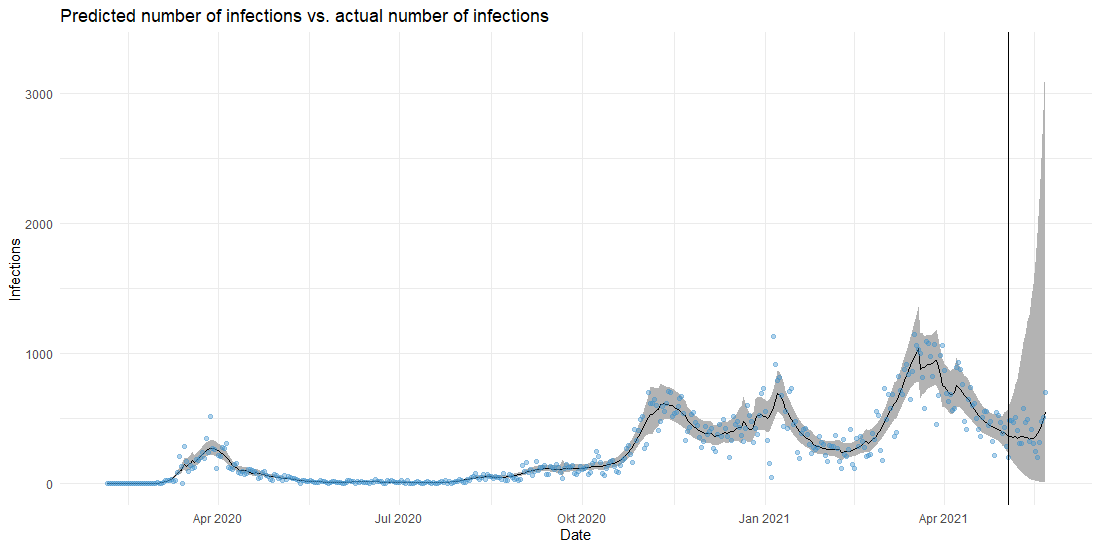
\includegraphics[width = 0.8\textwidth]{predictions_1_norway.png}
  \caption{The predicted number of infections in Norway according to the temporal model. The vertical line indicates where the test data begins.}
  \label{predictions_1_norway}
\end{figure}
\begin{figure}[H]
  \centering
  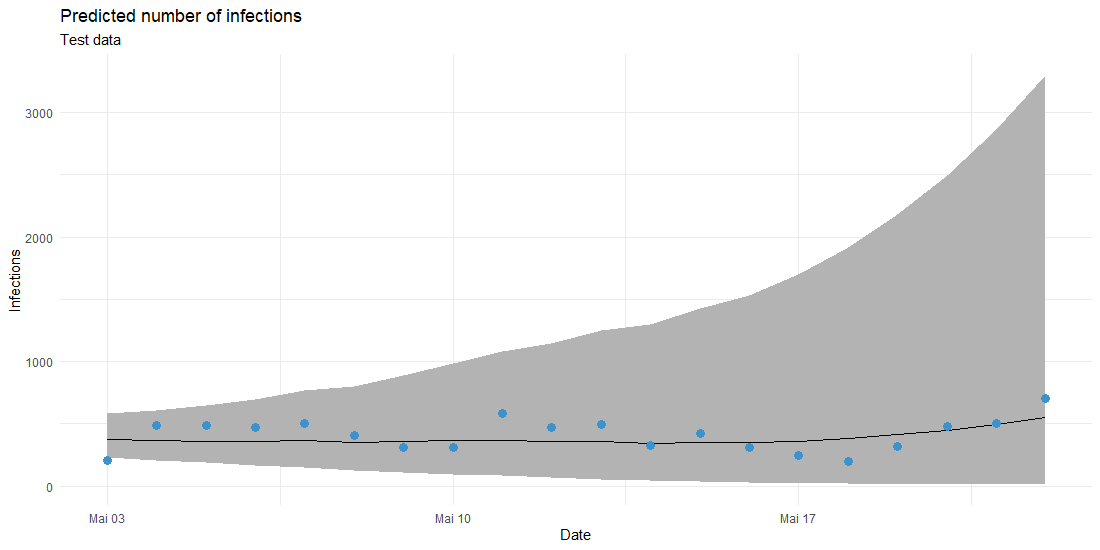
\includegraphics[width = 0.8\textwidth]{predictions_2_norway.png}
  \caption{The predicted number of infections in Norway according to the temporal model.}
  \label{predictions_2_norway}
\end{figure}
Comparing the 7-day incidence of the predicted data and the actual data in Figure~\ref{incidence_norway}, the incidences of the training data and the actual data follow the same pattern. However, the predicted 7-day incidence for the test data initially falls before rising, while the actual 7-day incidence initially rises and then falls before rising again. Although still not ideal, the predicted incidence for Norway looks slightly better than that for Germany, which can be seen in Figure~\ref{incidence_germany}.
\begin{figure}[H]
  \centering
  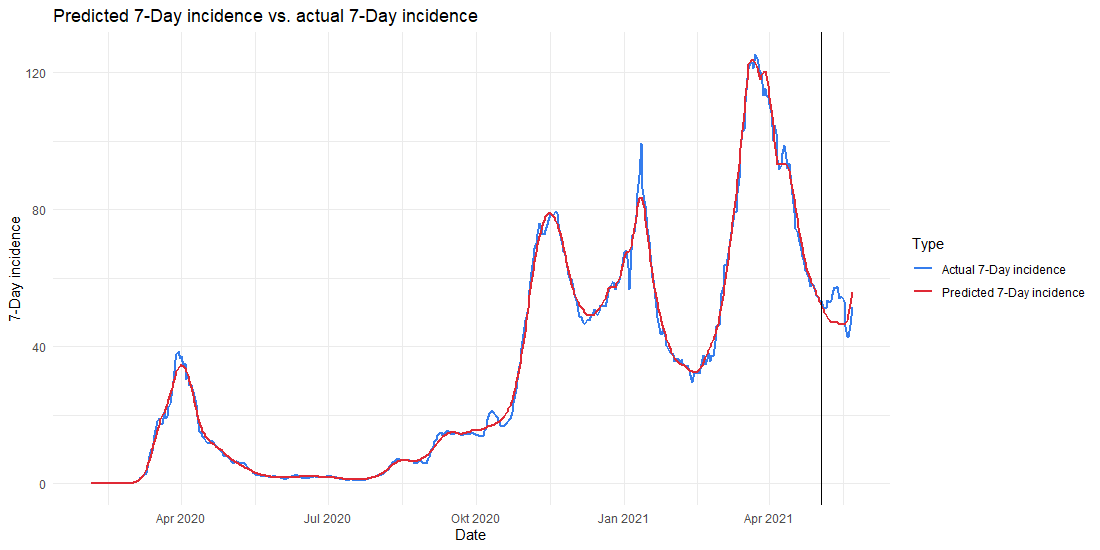
\includegraphics[width = 0.8\textwidth]{incidence_norway.png}  
  \caption{The 7-day incidence of the actual number of infections and the predicted number of infections. The vertical line indicates where the test data begins.}
  \label{incidence_norway}
\end{figure}
The posterior temporal trend for Norway in Figure~\ref{trend_norway} clearly shows all three waves, including the double peak of the second wave. It can also be seen that the third wave is clearly the worst in terms of infection numbers. On the other hand, however, the first and second waves appear to be equally bad in this graphic, while in reality the second wave in Norway was worse than the first. Just as with Germany in Figure~\ref{trend_germany}, a steep increase sets in after the third wave.
\begin{figure}[H]
  \centering
  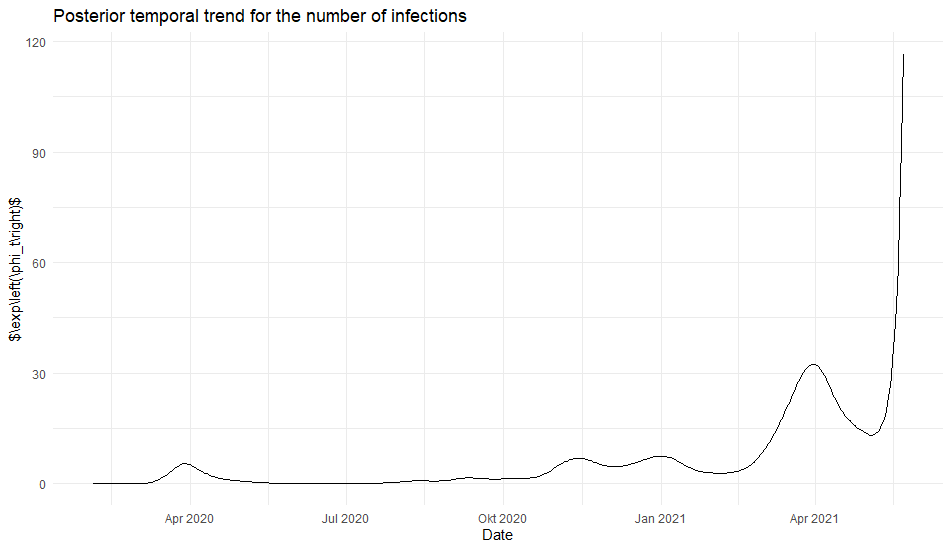
\includegraphics[width = 0.8\textwidth]{temp_trend_norway.png}  
  \caption{The posterior temporal trend for the number of infections.}
  \label{trend_norway}
\end{figure}
The covariates of the model are presented in Table~\ref{fixed_norway_temporal}. Apart from the intercept, the only significant effect is the mobility at workplaces.
\begin{table}[H]
\caption{The fixed effects for the model. Values are rounded. A $^*$ denotes a significant effect. \label{fixed_norway_temporal}}
\begin{tabular}{l r r r r c}
\toprule
\textbf{Variable}	& \textbf{mean$_{\hbox{p}}$}	& \textbf{exp(mean$_{\hbox{p}}$)} & \textbf{exp(q0025$_{\hbox{p}}$)} & \textbf{exp(q0975$_{\hbox{p}}$)} & \textbf{sig.}\\
\midrule
(Intercept) & -0.926 & 0.408 & 0.249 & 0.631 & $^*$ \\
Workplace mobility & 0.179 & 1.201 & 1.011 & 1.417 & $^*$ \\
Season winter & 0.109 & 1.159 & 0.645 & 1.924 \\
Main variant & 0.056 & 1.073 & 0.760 & 1.482 \\
Variant 20E & 0.041 & 1.043 & 0.942 & 1.149 \\
Restrictions internal & \multirow{3}{*}{0.012} & \multirow{3}{*}{1.063} & \multirow{3}{*}{0.545}& \multirow{3}{*}{1.854}\\
movement \\
Recommended \\
Stay home & \multirow{3}{*}{-0.058} & \multirow{3}{*}{1.033} & \multirow{3}{*}{0.413}& \multirow{3}{*}{2.163}\\
requirements \\
Recommended \\
Mobility grocery & \multirow{2}{*}{-0.081} & \multirow{2}{*}{0.923} & \multirow{2}{*}{0.831}& \multirow{3}{*}{1.022}\\
and pharmacy \\
Variant 20L & -0.086 & 0.963& 0.499 & 1.684 \\
Season spring & -0.089 & 0.962 &0.489 & 1.706 \\
season summer & -0.178 & 0.886 & 0.436 & 1.624\\
Restrictions internal & \multirow{3}{*}{-0.209} & \multirow{3}{*}{0.842}& \multirow{3}{*}{0.477}& \multirow{3}{*}{1.384} \\
movement \\
Movement restricted \\
\bottomrule
\end{tabular}
\end{table}